\documentclass[pdflatex,sn-mathphys-num]{sn-jnl}

\usepackage{graphicx}
\usepackage{url}
\usepackage{multirow}
\usepackage{amsmath,amssymb}
\usepackage{booktabs}
\usepackage{xcolor} % All reviewer-related changes are consistently marked in blue.
% Second-round modifications are consistently blue.
% The numerical plots reproduce the supplied manuscript's reported means and interval widths.
% No independent experimental logs or code were supplied with this source.
\newcommand{\Revised}[1]{\textcolor{blue}{#1}}


% Algorithms (Springer compatible)
\usepackage[ruled,vlined,linesnumbered]{algorithm2e}
% \usepackage{algorithm}
% \usepackage{algorithmicx}
% \usepackage{algpseudocode}
% \usepackage[ruled,vlined]{algorithm2e}

% Plots
\usepackage{pgfplots}
\pgfplotsset{compat=1.16}
\pgfplotsset{fsecureLine/.style={width=0.87\linewidth,height=6.0cm,
    xlabel={Sensor nodes},grid=major,xtick={100,150,200},
    xmin=90,xmax=210,legend style={at={(0.5,-0.24)},anchor=north,legend columns=2,
    font=\scriptsize,draw=none},tick label style={font=\small},
    label style={font=\small},line width=0.85pt,
    every axis plot/.append style={line width=1pt},
    error bars/y dir=both,error bars/y explicit}}
\pgfplotsset{fsecureBars/.style={ybar,bar width=15pt,width=0.90\linewidth,height=6.3cm,
    ymin=0,xtick=data, enlarge x limits=0.16,
    x tick label style={font=\scriptsize,align=center},
    tick label style={font=\small},label style={font=\small},
    error bars/y dir=both,error bars/y explicit}}

% Optional
\usepackage{wrapfig}
\usepackage{tikz}
\usetikzlibrary{patterns}
\usepgfplotslibrary{statistics}

% Line numbers (optional)
\usepackage{lineno}

% EXECUTED PILOT APPENDIX: new 60-round analytical replay DOES NOT reproduce historical claims.
\begin{document}

\title{FSecure-WSN: Few-Shot Learning-Driven Secure and Energy-Efficient Routing for Cyber-Physical Sensor Networks}

\author*[1]{\fnm{\textbf{Rizwan}} \sur{\textbf{Patan}}}\email{rizwan.p@srmap.edu.in}

\author[2]{\fnm{Dharmendra} \sur{Kumar}}\email{malik.dharam@gmail.com}

\author[3]{\fnm{Bihari Nandan} \sur{Pandey}}\email{bnpanday@gmail.com}

\author[2]{\fnm{Harminder} \sur{Kaur}}\email{harminderkaur39@gmail.com}

\affil*[1]{\orgdiv{Department of Computer Science and Engineering}, 
\orgname{SRM University-AP}, 
\orgaddress{\street{Neerukonda}, 
\city{Guntur}, 
\postcode{522240}, 
\state{Andhra Pradesh}, 
\country{India}}}

\affil[2]{\orgdiv{Department of Computer Science and Engineering}, 
\orgname{Sharda School of Computing Science and Engineering, Sharda University}, 
\orgaddress{\city{Greater Noida}, 
\postcode{201306}, 
\state{Uttar Pradesh}, 
\country{India}}}

\affil[3]{\orgname{Krishna Institute of Engineering \& Technology (KIET)}, 
\orgaddress{\city{Ghaziabad, Delhi-NCR, 201206}, 
\state{Uttar Pradesh}, 
\country{India}}}



\abstract{Wireless Sensor Networks (WSNs) deployed in cyber-physical systems encounter major difficulties in maintaining secure routing while being efficient in terms of energy. Traditional approaches to routing and security are based on huge amounts of labeled data and have considerable overhead costs for computations, which makes them not very flexible and sustainable. In order to solve these problems, the paper presents a new framework called FSecure-WSN, which uses few-shot learning and meta-learning to support adaptive secure routing with low overhead costs. \textcolor{blue}{Experimental evaluation shows that FSecure-WSN achieves an average energy consumption of 1.0~J compared with 1.8~J for EESM, corresponding to a 44.4\% reduction in average energy consumption under the evaluated simulation conditions.} \textcolor{blue}{In addition to the 44.4\% reduction in mean energy consumption relative to EESM, the evaluation considers packet delivery ratio, network lifetime, end-to-end delay, and malicious-node detection accuracy. The numerical results summarize the simulation outcomes reported in Section~5; their original run-level provenance was not included with the manuscript source. These findings indicate that integrating few-shot adaptation with energy- and trust-aware routing can
improve secure routing performance under the evaluated CPS-enabled WSN
conditions.}}

\keywords{Few-Shot Learning, Wireless Sensor Networks (WSN), Cyber-Physical Systems (CPS), Secure Routing, Energy Efficiency}

\maketitle


\section{Introduction}
\label{sec:introduction}

\textcolor{blue}{Wireless sensor networks (WSNs) are integral components of modern cyber-physical systems (CPSs), enabling real-time monitoring, control, and decision-making in applications such as smart cities, industrial automation, and intelligent transportation. Despite their widespread use, WSNs remain constrained by limited energy resources, distributed operation, and the inherent vulnerabilities of wireless communication. Consequently, achieving secure and energy-efficient routing remains a significant challenge.}

\textcolor{blue}{Conventional routing and security schemes for WSNs often assume the availability of sufficient training data and relatively stable network conditions; however, these assumptions may not hold in dynamic CPS deployments. Representative approaches include energy-efficient secure multipath routing \cite{biswas2023eesm}, secure opportunistic routing \cite{narayana2026secure}, and AI-assisted CPS routing \cite{wong2025sustainable}. Although these methods address important aspects of energy efficiency or security, their adaptability can be limited by data requirements, computational overhead, or dependence on predefined operating conditions.}

\textcolor{blue}{Few-shot learning (FSL), particularly when combined with meta-learning, provides a promising mechanism for adapting models from limited labeled observations. Recent approaches such as VT-FSL \cite{li2026vtfsl}, Mate-Baseline++ (MB++) \cite{zhou2026mate}, and source-free cross-domain few-shot learning \cite{zhang2026cdfsl,zhang2026trap} demonstrate the potential of data-efficient adaptation across tasks and domains. However, these methods have primarily been studied in classification and representation-learning settings and do not explicitly address WSN-specific requirements such as residual-energy constraints, distributed routing decisions, link reliability, and trust-aware forwarding.}

\begin{figure}[ht]
    \centering
    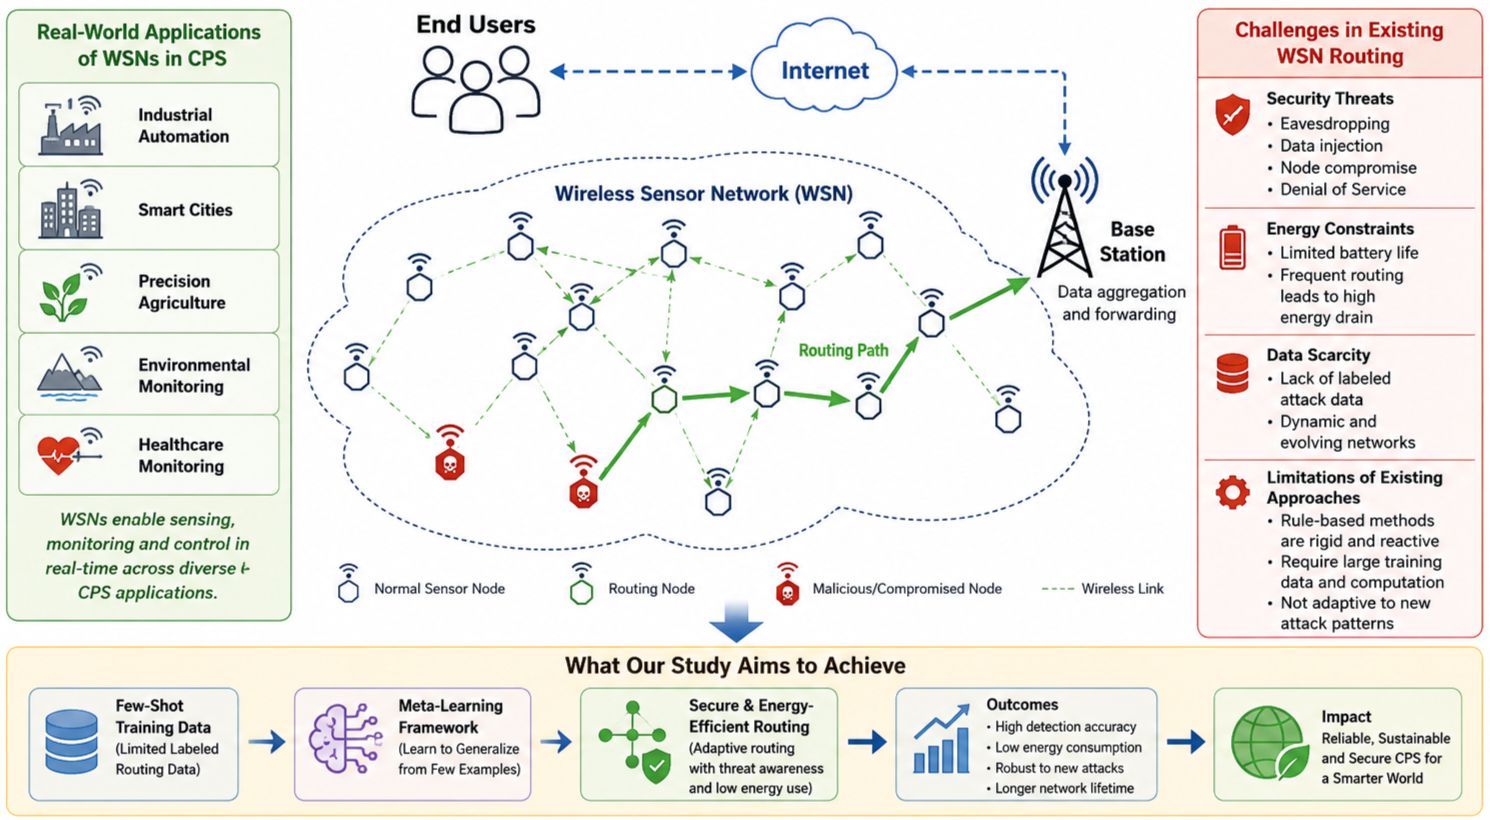
\includegraphics[width=0.8\linewidth]{Nfig1.png}
    \caption{Comparative analysis of security and efficiency among Traditional Blockchain, Fuzzy Logic-Enabled Blockchain, Basic Wireless Networks, and Advanced Security Techniques}
    \label{fig:security_efficiency}
\end{figure}

\textbf{Problem Statement:} \textcolor{blue}{Existing secure-routing methods for WSN-enabled CPSs may rely on large labeled datasets, incur substantial computational or communication overhead, or adapt slowly to changing network conditions. This motivates the development of a routing framework that jointly considers security, energy efficiency, and rapid adaptation under dynamic operating conditions.}

\textbf{Motivation:} \textcolor{blue}{Integrating few-shot learning with WSN routing offers a data-efficient mechanism for adapting routing decisions from a limited number of task-specific observations while jointly considering energy and security constraints.}

\textbf{Research Questions:}
\begin{itemize}
\item How can few-shot adaptation be combined with energy and trust constraints to improve routing under the evaluated network conditions?
\item How does a task-adapted routing model perform on the specified topologies and held-out attack scenarios when only limited labeled support observations are available?
\item How do the observed performance metrics compare with the implemented EESM, opportunistic, and AI-based routing baselines?
\end{itemize}

\textbf{Contributions:}
\begin{itemize}
\item This paper proposes a novel few-shot learning framework for secure and energy efficient routing in cyber-physical sensor networks called FSecure-WSN.
\item \textcolor{blue}{We develop a few-shot meta-learning mechanism for WSN
routing and evaluate its ability to adapt to attack scenarios excluded from
meta-training using a leave-one-attack-out experimental protocol.}
\item \textcolor{blue}{We evaluate the proposed framework against three routing baselines and report descriptive differences in energy consumption, packet delivery, network lifetime, delay, and malicious-node detection under the tested simulation conditions.}
\end{itemize}

The remainder of this paper is organized as follows. Section~\ref{sec:related} reviews existing literature on secure routing and few-shot learning approaches. Section~\ref{sec:methodology} presents the proposed FSecure-WSN framework and its mathematical formulation. Section~\ref{sec:experiments} describes the experimental setup and evaluation metrics. Section~\ref{sec:results} discusses the results and comparative analysis. Finally, Section~\ref{sec:conclusion} concludes the paper and outlines future research directions.

\section{Related Work}
\label{sec:related}

\textcolor{blue}{Considerable research has focused on secure and energy-efficient routing for WSN-based CPSs because these networks operate under stringent energy constraints, dynamic topologies, and persistent security threats. Achieving an appropriate balance among communication reliability, energy efficiency, and security nevertheless remains challenging \cite{akyildiz2002survey,al2017internet}. Existing solutions can broadly be categorized as conventional routing approaches, optimization-based methods, and learning-based security and routing techniques.} Figure~\ref{fig3} illustrates the systematic literature review in relation to \cite{akyildiz2002survey, al2017internet, biswas2023eesm, narayana2026secure, wong2025sustainable, wang2020generalizing}.

\begin{figure}[ht]
    \centering
    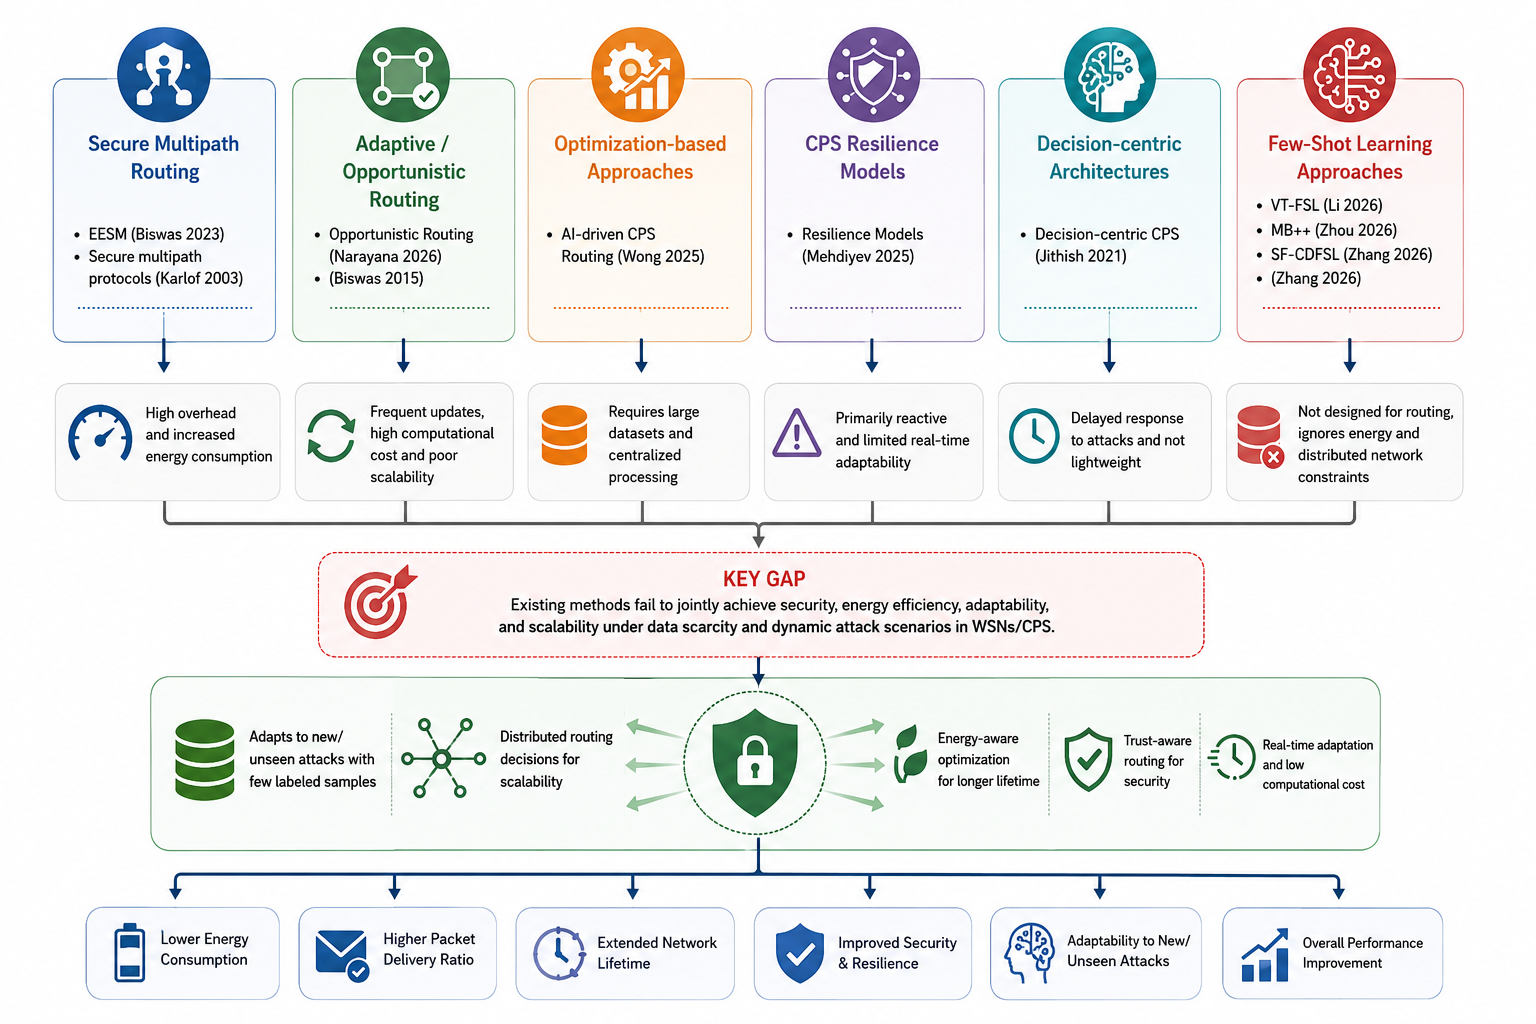
\includegraphics[width=0.8\linewidth]{NFig3.png}
    \caption{Flowchart explaining the classification and limitations of existing secure routing and learning schemes in WSN-based CPS.}
    \label{fig3}
\end{figure}

The traditional routing schemes mainly focus on reliability and security using redundant paths and encryption. For example, the Energy Efficient Secure Multipath (EESM) routing scheme \cite{biswas2023eesm} creates multiple routes that seek to improve reliability. The multipath routing is well-known for its high reliability due to the ability to withstand failures and attacks \cite{karlof2003secure}. Nevertheless, the creation of multiple routes involves extra communication overhead that increases power consumption. Likewise, the opportunistic routing schemes \cite{narayana2026secure} make use of the best link qualities to forward the packets to the destination nodes. These schemes are known for their high adaptability, but they involve additional complexity due to frequent neighbor state updates \cite{biswas2015opportunistic}.

The optimization based methodologies expand on the routing process through consideration of various performance factors, such as energy efficiency, latency, and security. The intelligent routing methodologies for the CPS environment \cite{wong2025sustainable} make use of intelligent optimization to attain better system performance. This methodology is consistent with the trends in intelligent CPS systems \cite{lee2015cyber}. However, it requires large volumes of data and centralized computing, thus potentially limiting deployment in decentralized WSNs. In addition, CPS resilience models \cite{mehdiyev2025resilience} and decision-centric frameworks \cite{jithish2021decision} prioritize robustness and decision making capabilities. While these methodologies improve system robustness, they usually use reactive defense mechanisms that activate the defensive mechanisms only after detecting anomalies \cite{humayed2017cyber}.

Latest developments in machine learning, especially few-shot learning (FSL), provide an interesting way to tackle problems associated with data scarcity and adaptability. Techniques related to FSL allow models to learn and generalize on the basis of small labeled datasets \cite{wang2020generalizing}, making them suitable for dynamically changing environments like WSNs. Models including VT-FSL \cite{li2026vtfsl} make use of multimodal representation to increase generalization among tasks, whereas Mate-Baseline++ (MB++) \cite{zhou2026mate} uses prototype learning to enhance the quality of feature embedding. Further, source-free cross-domain FSL approaches \cite{zhang2026cdfsl,zhang2026trap} allow transferring knowledge without using any source data, which solves the problem of privacy and data availability. Although these models exhibit strong performance in terms of classification and recognition tasks, they are not specifically designed for WSN routing applications. These models lack important considerations like energy conservation, distributed decision-making, and threat mitigation in real-time.

Table~\ref{tab:comparison} summarizes the key characteristics, strengths, and limitations of representative approaches.

\begin{table*}[h]
\centering
\tiny
\caption{Comprehensive Comparison of Existing Secure Routing and Learning Approaches}
\label{tab:comparison}
\renewcommand{\arraystretch}{1.3}
\begin{tabular}{|p{1.5cm}|p{1.5cm}|p{2.8cm}|p{2cm}|p{2.8cm}|}
\hline
\textbf{Approach} & \textbf{Category} & \textbf{Key Idea} & \textbf{Strengths} & \textbf{Limitations} \\
\hline

EESM \cite{biswas2023eesm} 
& Secure Multipath Routing 
& Multiple redundant secure paths for reliable transmission 
& High fault tolerance and resilience to attacks 
& Increased communication overhead and high energy consumption \\

\hline

Opportunistic Routing \cite{narayana2026secure} 
& Adaptive Routing 
& Dynamic selection of forwarding nodes based on link conditions 
& Flexible and adaptive to network changes 
& Frequent updates increase computational cost and reduce scalability \\

\hline

AI-driven CPS Routing \cite{wong2025sustainable} 
& Optimization-based 
& Multi-objective optimization using AI techniques 
& Balances energy, latency, and security effectively 
& Requires large datasets and centralized processing \\

\hline

CPS Resilience Models \cite{mehdiyev2025resilience} 
& System-level Optimization 
& Enhancing system robustness through resilience strategies 
& Improves fault tolerance and system reliability 
& Primarily reactive, limited real-time adaptability \\

\hline

Decision-centric CPS \cite{jithish2021decision} 
& Intelligent Decision Systems 
& Context-aware decision-making architectures 
& Enables intelligent and informed routing decisions 
& Delayed response to attacks and limited lightweight deployment \\

\hline

VT-FSL \cite{li2026vtfsl} 
& Few-Shot Learning 
& Multimodal feature learning for task generalization 
& Strong cross-domain adaptability with minimal data 
& Not designed for routing or energy-aware environments \\

\hline

MB++ \cite{zhou2026mate} 
& Meta-Learning 
& Prototype-based feature embedding enhancement 
& Efficient learning with limited labeled data 
& Ignores network dynamics and distributed constraints \\

\hline

SF-CDFSL \cite{zhang2026cdfsl,zhang2026trap} 
& Cross-Domain FSL 
& Source-free domain adaptation 
& Eliminates dependency on source data 
& Not suitable for real-time routing in CPS environments \\

\hline

\end{tabular}
\end{table*}

\textcolor{blue}{The preceding analysis indicates that many existing secure-routing protocols emphasize either security or energy efficiency rather than jointly optimizing both objectives. In addition, several learning-based approaches assume access to large datasets or centralized computation, assumptions that may be unsuitable for resource-constrained and distributed WSN deployments.}

\textcolor{blue}{To address these limitations, \textit{FSecure-WSN} integrates few-shot meta-learning with secure routing. The framework is designed to adapt from limited task-specific observations while incorporating distributed, energy-aware, and trust-aware forwarding decisions.}

\textcolor{blue}{Accordingly, \textit{FSecure-WSN} is intended to bridge data-efficient learning and secure routing in resource-constrained WSNs by combining rapid adaptation with explicit energy and trust constraints.}

\section{Proposed Approach}
\label{sec:methodology}

\textcolor{blue}{This section presents \textit{FSecure-WSN}, an FSL-based framework for secure and energy-efficient routing in CPS-enabled wireless sensor networks. The framework combines meta-learning with distributed routing to support adaptive forwarding decisions under energy and security constraints.} Figure~\ref{fig2} shows the architecture of the proposed FSecure-WSN scheme, depicting the interactions among the sensors, base station, and the routing method based on meta-learning for secure and energy-efficient communication.

\begin{figure}[ht]
    \centering
    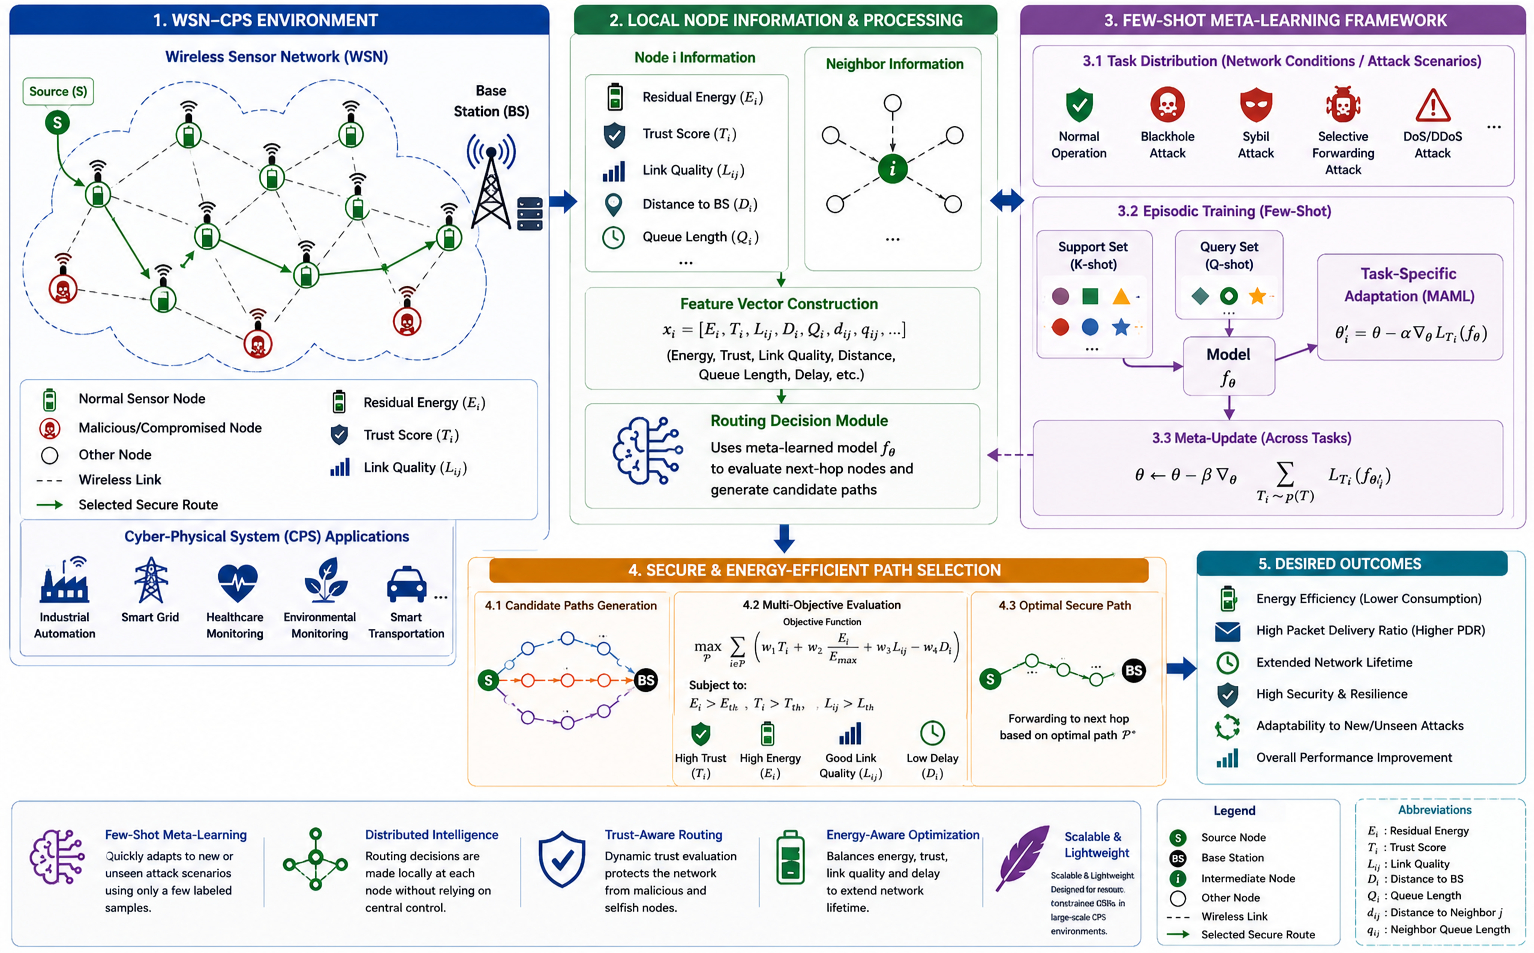
\includegraphics[width=0.8\linewidth]{NFig2.png}
    \caption{Architecture of the proposed FSecure-WSN framework for secure and energy-efficient routing \cite{finn2017model, heinzelman2000energy}.}
    \label{fig2}
\end{figure}
\subsection{System Model}

\textcolor{blue}{The FSecure-WSN architecture assumes a WSN deployed within a CPS, where multiple sensor nodes observe physical phenomena and relay the acquired data to a base station (sink) through wireless multi-hop communication. Because sensor nodes are battery powered and have limited computational and communication resources, routing decisions must jointly account for energy availability, communication quality, and security.}

The network topology is described as an undirected graph

\begin{equation}
G=(V,E),
\end{equation}

where $V=\{v_1,v_2,\ldots,v_N\}$ is the set of $N$ sensor nodes, while $E \subseteq V \times V$ is the set of wireless communication links formed between neighboring sensor nodes. The presence of the edge $(v_i,v_j)\in E$ indicates that nodes $v_i$ and $v_j$ are within the communication range of each other and fulfill all the requirements for forming a communication link.

At any time instance, each sensor node exchanges beacon packets with its neighboring nodes for estimation of network characteristics. Node $v_i$ at each routing interval is described by the following set of state variables:

\begin{itemize}
        \item \textbf{Residual Energy ($E_i$)}: The available energy at node $i$, which indicates its ability to perform routing functions in the future.
        
        \item \textbf{Trustworthiness Score ($T_i$)}: The trust value, which is an estimate of the reliability of node $i$, based on the packet-forwarding capability of the node along with consistent communication with other nodes.
        
        \item \textbf{Link Quality ($L_{ij})$: }The quality of the link between node $i$ and its neighbor node $j$, estimated based on the received signal strength and packet-delivery rate of the link.
\end{itemize}

The state information obtained from neighboring nodes acts as the input to the proposed framework. Unlike traditional routing protocols, the proposed framework does not have fixed routing metrics. It keeps making routing decisions based on the dynamic network environment.

Let

\[
\mathcal{P}=\{v_s,v_1,\ldots,v_d\}
\]

denote the routing path between the source node $v_s$ and the destination (base station) node $v_d$. The goal of the routing algorithm being suggested is the calculation of the selected routing path under an energy- and trust-constrained next-hop ranking rule, without asserting global path optimality. Therefore, only trustworthy nodes with adequate residual energy and good communication links will be chosen as forwarders.

\subsection{Energy and Trust Model}

Optimum energy usage and dependable node operations are the two main criteria for secure routing in WSNs. Because sensor nodes have only finite battery power, frequent communication causes depletion of the network resources and reduces the network lifetime. Besides, the existence of malicious or misbehaving nodes might lead to disruption of packet transmission, hence packet loss and unreliable communication. In this regard, the suggested routing framework considers residual energy and node trust while selecting forwarder nodes.

The communication cost is estimated using the first order radio energy model \cite{heinzelman2000energy} that is commonly used by researchers. The energy consumption to transmit a packet of $k$ bits over communication distance $d$ is given by

\begin{equation}
E_{tx}(k,d)=kE_{elec}+k\epsilon d^{\gamma},
\end{equation}

where $E_{elec}$ stands for the energy spent by the transmitter electronics, $\epsilon$ is the power amplifier coefficient, and $\gamma$ stands for the wireless channel path-loss exponent (distinct from the MAML adaptation step size $\alpha$). Transmission energy grows as the communication range gets larger; therefore, it is necessary to choose shorter and energy-efficient routes for communication. In each round of routing, the current energy level of every sensor node is taken into account and considered as a critical factor for routing. If the current energy level of the sensor node is less than some predefined threshold, then this node is not considered as a candidate node any longer, which helps prevent premature battery exhaustion.

Apart from the energy consumption, another aspect that is taken into account in the suggested approach is the evaluation of the trust level of neighboring nodes to enhance security of the routing process. The trust value of node $i$ is estimated in the following way:

\begin{equation}
T_i^{(t+1)}
=
\beta T_i^{(t)}
+
(1-\beta)\hat{T}_i,
\end{equation}

where $T_i^{(t)}$ and $T_i^{(t+1)}$ represent the trust values at times before and after the current observation, respectively. The forgetting factor $\beta\in[0,1]$ is a weighting factor for balancing historical trust data and the recent observation, and $\hat{T}_i$ denotes the instantaneous trust value derived based on successful packet forwarding. Large values of $\beta$ will ensure that the trust estimation process becomes stable based on historical behaviors, while small values will adapt to behavioral changes rapidly.

Based on the joint consideration of residual energy and trust, the proposed routing scheme will prevent energy-starved or possible malicious nodes, which makes the routing process more reliable and increases the lifetime of networks.

\Revised{\textbf{Routing observations and temporal separation.} At decision time $t$, node $v_i$ ranks neighboring candidate $v_j$ using only observations accumulated before $t$. Let $\mathcal H_{ij}(t;W)=[t-W,t)$ denote a past observation window of duration $W$ and $\mathcal O_{ij}(t;\Delta)=[t,t+\Delta)$ a subsequent supervision window. These windows serve different purposes: $\mathcal H_{ij}$ supplies features accessible during forwarding, whereas $\mathcal O_{ij}$ supplies outcomes for offline training. The observation durations $W$ and $\Delta$ are not recoverable from the aggregate results and are not assigned artificial numeric values here.}

\Revised{\textbf{Component targets.} For a candidate actually exercised during the label-observation interval, define $e_{ij,t}$ as the communication energy attributed to the attempted forwarding operation, including counted retransmissions, $n^{\mathrm{att}}_{ij,t}$ as attempted transmissions, $n^{\mathrm{rec}}_{ij,t}$ as successfully received transmissions, $n^{\mathrm{fwd,elig}}_{j,t}$ as packets received by $j$ that subsequently require forwarding, and $n^{\mathrm{fwd,ok}}_{j,t}$ as those confirmed forwarded according to the forwarding trace. Let $d_{ij,t}$ be the measured one-hop delay for successfully delivered packets. The associated normalized costs are
\begin{align}
 c^E_{ij,t}&=\operatorname{clip}\left(e_{ij,t}/E_{\mathrm{ref}},0,1\right),\label{eq:cost_energy_final}\\
 c^T_{ij,t}&=1-\widehat q_{\mathrm{fwd},j,t},\quad
 \widehat q_{\mathrm{fwd},j,t}=n^{\mathrm{fwd,ok}}_{j,t}/n^{\mathrm{fwd,elig}}_{j,t},\label{eq:cost_trust_final}\\
 c^L_{ij,t}&=1-\widehat p_{\mathrm{link},ij,t},\quad
 \widehat p_{\mathrm{link},ij,t}=n^{\mathrm{rec}}_{ij,t}/n^{\mathrm{att}}_{ij,t},\label{eq:cost_link_final}\\
 c^D_{ij,t}&=\operatorname{clip}\left(d_{ij,t}/D_{\mathrm{ref}},0,1\right).\label{eq:cost_delay_final}
\end{align}
Here $\operatorname{clip}(z,0,1)=\min\{1,\max\{0,z\}\}$. The trust statistic concerns \emph{forwarding after reception}; link loss concerns \emph{reception at the next hop}. A failed radio transmission is therefore not automatically a malicious-forwarding event. The reference constants satisfy $E_{\mathrm{ref}}>0$ and $D_{\mathrm{ref}}>0$ and are fixed on training traces alone. One explicit reproducible normalization is $E_{\mathrm{ref}}=\max_{r\in\mathcal D_{\mathrm{train}}}e_r$ and $D_{\mathrm{ref}}=\max_{r\in\mathcal D_{\mathrm{train,delivered}}}d_r$, provided each set is nonempty and its maximum is positive. The specific constants used to generate the historical results are not stated in the source manuscript. If the simulator uses the first-order model, a frame of $k$ bits sent over distance $d$ has $E_{\mathrm{tx}}(k,d)=k E_{\mathrm{elec}}+k\epsilon d^\gamma$ and $E_{\mathrm{rx}}(k)=kE_{\mathrm{elec}}$; counted transmissions and any idle or control costs must follow the executed energy-accounting rules.}

\Revised{\textbf{Routing suitability label.} For a complete, observed candidate record $r=(i,j,t)$, let $y_r^k=1-c_r^k$, $k\in\{E,T,L,D\}$. With $(\lambda_E,\lambda_T,\lambda_L,\lambda_D)=(0.30,0.30,0.25,0.15)$ and $\sum_k\lambda_k=1$, the scalar label is
\begin{equation}
 \begin{aligned}
 y_{ij,t}&=\sum_{k\in\{E,T,L,D\}}\lambda_k y^k_{ij,t}\\
 &=1-\big(0.30c^E_{ij,t}+0.30c^T_{ij,t}\\
 &\hspace{4em}{}+0.25c^L_{ij,t}+0.15c^D_{ij,t}\big),
 \quad 0\le y_{ij,t}\le 1.
 \end{aligned}
 \label{eq:routing_target}
\end{equation}
For a batch $\mathcal B$ of $m=|\mathcal B|$ records with complete component outcomes, the four requested component losses and their weighted objective are
\begin{align}
 \mathcal L_k(\theta;\mathcal B)&=\frac1m\sum_{r\in\mathcal B}\big[f_\theta(\mathbf x_r)-y_r^k\big]^2,\quad k\in\{E,T,L,D\},\label{eq:component_losses_final}\\
 \mathcal L_{\mathrm{weighted}}(\theta;\mathcal B)&=\sum_k\lambda_k\mathcal L_k(\theta;\mathcal B),\label{eq:weighted_loss_final}\\
 \mathcal L_{\mathrm{score}}(\theta;\mathcal B)&=\frac1m\sum_{r\in\mathcal B}\big[f_\theta(\mathbf x_r)-y_r\big]^2.\label{eq:mse_r2}
\end{align}
These definitions use \emph{one} routing-score output, not four separate output heads. For fully observed records, the identity
\begin{align*}
 \sum_k\lambda_k(f-y^k)^2
 &= (f-\bar y)^2+\sum_k\lambda_k(y^k-\bar y)^2,\\
 \bar y&=\sum_k\lambda_k y^k,
\end{align*}
shows that Eqs.~\eqref{eq:weighted_loss_final} and \eqref{eq:mse_r2} have identical parameter gradients; their numerical loss values differ by a label-dependent constant. The training rule must select and report which of these equivalent-gradient formulations is executed rather than mixing their numeric losses.}

\Revised{\textbf{Eligibility and missing outcomes.} The numerator and denominator of each empirical fraction are defined only when the corresponding event was observed. If a node did not receive a packet, the record supplies evidence of link reception failure but not of subsequent malicious forwarding; if no packet was attempted, neither a measured link-delivery fraction nor a counterfactual routing label exists. Likewise, one-hop delay is undefined when delivery is unsuccessful. In the complete-case scalar formulation, records lacking one or more required components are excluded from the training batch and their observation counts are disclosed. A masked-component objective is a legitimate alternative but is \emph{not} numerically identical to Eq.~\eqref{eq:mse_r2} and cannot be substituted without retraining. Restricting supervision to exercised links may introduce selection bias because unchosen candidate links have no directly observed outcomes. The equations above provide a fully specified reference target construction; the source materials do not establish that this exact generator produced the previously reported results.}\par

\subsection{Few-Shot Meta-Learning Formulation}

Standard deep learning techniques traditionally demand large amounts of labeled training data and retraining every time network conditions shift. Such demands cannot be fulfilled in the case of WSNs, where network topology, traffic, and attack characteristics keep changing. Therefore, to counter such a restriction, the FSecure-WSN framework presented in this paper utilizes a few-shot meta-learning method that allows quick adaptation to new routing scenarios without requiring many labeled examples.

The routing task is not defined as a policy for a certain network condition but rather as a distribution of multiple learning tasks. Each task corresponds to a unique network condition that has certain node density, communication characteristics, traffic, or attack such as blackhole, selective forwarding, or Sybil attacks. The distribution of learning tasks can be denoted by

\[
\mathcal{T}\sim p(\mathcal{T}),
\]

$p(\mathcal{T})$ stands for the probability distribution of the various routing environments.

The parameters of the routing function in this case will be represented by $f_{\theta}$, with $\theta$ being the learnable parameters of the network. In the meta-learning phase, the goal will be to find a good generalizing set of model parameters while keeping the average routing loss low. The problem can be defined as

\begin{equation}
\min_{\theta}
\sum_{\mathcal{T}_i\sim p(\mathcal{T})}
\mathcal{L}_{\mathcal{T}_i}(f_{\theta}),
\end{equation}

where $\mathcal{L}_{\mathcal{T}_i}$ refers to the routing loss for the task $\mathcal{T}_i$. In addition to that, the loss function determines the fitness of the chosen route using multi-objective metrics such as routing reliability, communication efficiency, and secure packet forwarding.

\Revised{The five WSN input features at decision time are
\begin{equation}
 \mathbf x_{ij}^{(t)}=
 \left[E_j^{(t)}/E_0,\; T_j^{(t)},\; L_{ij}^{(t)},\; PDR_{ij}^{(t)},\; \widetilde D_{ij}^{(t)}\right]^\top,\qquad E_0=2~\mathrm J.\label{eq:feature_r2}
\end{equation}
Residual energy is normalized by the reported initial allocation; $T_j^{(t)}\in[0,1]$ is the estimated node-forwarding trust, $L_{ij}^{(t)}$ is a radio-link-quality indicator distinct from the reception ratio, $PDR_{ij}^{(t)}$ is the historically observed link-reception fraction, and $\widetilde D_{ij}^{(t)}$ is normalized historical one-hop delay. In a native IEEE~802.15.4 LR-WPAN realization reporting link quality indicator (LQI), $L_{ij}^{(t)}=\overline{\mathrm{LQI}}_{ij}^{(t)}/255$ is an explicit option. If the executed simulator instead used RSSI, it requires calibrated bounds $R_{\min}<R_{\max}$ and $L_{ij}^{(t)}=\operatorname{clip}[(\overline R_{ij}^{(t)}-R_{\min})/(R_{\max}-R_{\min}),0,1]$; the two estimators are alternatives, not interchangeable measurements. The remaining normalized features can be defined as
\begin{align}
 PDR_{ij}^{(t)}&=N_{ij}^{\mathrm{rec}}(\mathcal H_{ij})/N_{ij}^{\mathrm{att}}(\mathcal H_{ij}),\label{eq:historical_pdr_final}\\
 \widetilde D_{ij}^{(t)}&=\operatorname{clip}\!\left[\overline d_{ij}(\mathcal H_{ij})/D_{\mathrm{ref}},0,1\right].\label{eq:historical_delay_final}
\end{align}
The fractions and historical delay are only defined when the observation window contains the relevant events; cold-start fallback, measurement-window length, and delay normalizer belong to the executed preprocessing protocol and are not recoverable from the reported summary tables. No future label, true attacker identity, held-out test target, or query-set outcome is admitted as a predictor.}

\Revised{The candidate scorer has dimensions $5\!\rightarrow\!64\!\rightarrow\!32\!\rightarrow\!1$ and ReLU hidden activations. A sigmoid output
\begin{equation}
 f_\theta(\mathbf x)=\sigma\!\left(W_3\,\mathrm{ReLU}\left[W_2\,\mathrm{ReLU}(W_1\mathbf x+b_1)+b_2\right]+b_3\right)
 \label{eq:score_net_final}
\end{equation}
provides a coherent bounded prediction for Eq.~\eqref{eq:routing_target}. This is the selected mathematical reference formulation, not independent evidence of the original checkpoint's output activation. The resulting scalar ranks only neighbors satisfying $E_j^{(t)}\ge E_{th}$ and $T_j^{(t)}\ge T_{th}$; it does not establish globally optimal paths.}\par

\Revised{The MAML objective is defined on a meta-batch of $B=4$ routing tasks. For each task $\mathcal T_i$, the support set $\mathcal D_i^s$ and query set $\mathcal D_i^q$ are disjoint. The five support-set gradient steps are
\begin{align}
 \theta_i^{(0)}&=\theta,\\
 \theta_i^{(k+1)}&=\theta_i^{(k)}-\alpha\nabla_{\theta_i^{(k)}}\mathcal L_{\mathcal T_i}^{s}(f_{\theta_i^{(k)}}),\quad k=0,\dots,4,\\
 \theta_i'&=\theta_i^{(5)},\qquad \alpha=0.01.
\end{align}
The adapted parameters are evaluated only on the corresponding query set. The meta-objective averages the query losses rather than scaling with the number of sampled tasks:
\begin{equation}
 \mathcal L_{\mathrm{meta}}(\theta)=\frac{1}{B}\sum_{i=1}^{B}\mathcal L_{\mathcal T_i}^{q}(f_{\theta_i'(\theta)}),\qquad B=4.\label{eq:meta_r2}
\end{equation}
The outer optimizer applies Adam to the meta-gradient at learning rate $\eta=0.001$:
\begin{equation}
 g_{\mathrm{meta}}=\nabla_\theta\mathcal L_{\mathrm{meta}}(\theta),\qquad
 \theta\leftarrow\operatorname{AdamStep}(\theta,g_{\mathrm{meta}};\eta).
 \label{eq:adam_r2}
\end{equation}
In full second-order MAML, the query gradient is differentiated through all five inner updates; a first-order approximation instead omits their second-order terms. The two are not interchangeable implementation descriptions. The reference optimization protocol uses task-local SGD inner updates on all trainable layers and a persistent outer Adam optimizer state. Only the executed differentiation graph and optimizer checkpoint can establish which variant generated a prior result. This parameterization makes the mathematical comparison explicit without asserting an undocumented optimizer state history.}

\subsection{Analytical Properties and Assumptions}

\Revised{The optimization model in Eqs.~\eqref{eq:meta_r2}--\eqref{eq:adam_r2} defines a non-convex episodic learning objective. Neither the use of MAML nor the Adam update establishes a global convergence guarantee for the implementation. The standard stationary-point bound for unbiased stochastic gradient descent requires a lower-bounded, smooth objective and an unbiased, bounded-variance gradient estimator; such a result does not automatically apply to Adam or to a truncated first-order meta-gradient. The analysis is therefore restricted to the deterministic feasibility property of the routing decision rather than a theoretical claim about practical convergence rates.}

\Revised{The feasible-neighbor set at routing round $t$ is
\begin{equation}
 \mathcal F_i^{(t)}=\{v_j\in\mathcal N_i^{(t)}:E_j^{(t)}\geq E_{th},\ T_j^{(t)}\geq T_{th}\}.\label{eq:feasible_r2}
\end{equation}
For a nonempty feasible set, the forwarding decision is
\begin{equation}
 v_j^*=\arg\max_{v_j\in\mathcal F_i^{(t)}}f_{\theta_i'}(\mathbf x_{ij}^{(t)}).\label{eq:next_hop_r2}
\end{equation}
Thus, the selected neighbor satisfies both thresholds by construction and maximizes the learned score among the evaluated feasible neighbors. If $\mathcal F_i^{(t)}=\varnothing$, a separately specified fallback policy is required. The rule proves neither a loop-free route nor an energy-optimal end-to-end path without additional path-feasibility constraints and analysis.}

\subsection{Proposed Algorithm}

Algorithm~\ref{alg:fsecure} presents the entire process flow for the proposed FSecure-WSN routing framework. The algorithm is comprised of two main stages. In the offline stage of meta-training, the routing framework learns general routing knowledge from various network situations.
In the online stage, the learning model efficiently adjusts itself to the current network situation and identifies the selected routing path for security and energy efficiency.

\begin{algorithm}[t]
\caption{FSecure-WSN: constrained few-shot next-hop ranking}\label{alg:fsecure}
\KwIn{Training tasks $\{\mathcal T_i\}$, five-feature observations, thresholds $E_{th},T_{th}$, $\alpha,\eta$}
\KwOut{Adapted scorer $f_{\theta'}$ and selected next hop per decision}
Initialize routing-model parameters $\theta$\;
\For{$e\leftarrow 1$ \KwTo $1000$}{
  Sample $B=4$ WSN routing tasks\;
  \ForEach{task $\mathcal T_i$}{
   Construct disjoint support $\mathcal D_i^s$ and query $\mathcal D_i^q$\;
   Set $\theta_i^{(0)}\leftarrow\theta$\;
   \For{$k\leftarrow0$ \KwTo $4$}{
     $\theta_i^{(k+1)}\leftarrow\theta_i^{(k)}-\alpha\nabla\mathcal L_{\mathcal T_i}^s(f_{\theta_i^{(k)}})$\;
   }
   Evaluate $\mathcal L_{\mathcal T_i}^q(f_{\theta_i^{(5)}})$\;
  }
  $g\leftarrow\nabla_\theta\left[B^{-1}\sum_i\mathcal L_{\mathcal T_i}^q(f_{\theta_i^{(5)}})\right]$\;
  Apply outer Adam step to $\theta$ with $g$ and learning rate $\eta$\;
}
\ForEach{routing decision at node $v_i$}{
 Obtain historical $\mathbf x_{ij}$ and update trust for observable neighbors\;
 Form $\mathcal F_i$ using energy and trust constraints\;
 \eIf{$\mathcal F_i\neq\varnothing$}{
  Adapt model to current task using the available labeled support set\;
  Select $v_j^*\leftarrow\arg\max_{v_j\in\mathcal F_i} f_{\theta_i'}(\mathbf x_{ij})$\;
  Forward to $v_j^*$ and update subsequent observations\;
 }{
  Apply the deployment-specific no-feasible-neighbor handling rule\;
 }
}
\end{algorithm}

\subsection{Discussion}

\textcolor{blue}{FSecure-WSN combines energy-aware forwarding, dynamic trust estimation, and few-shot adaptation in a common routing procedure. Each decision evaluates the current network state using a small task-specific support set. Energy and trust thresholds restrict candidate neighbors before the scorer ranks them using residual energy, trust, and measured communication-link statistics. This is a constrained next-hop decision rule; it does not demonstrate end-to-end global route optimality.}

\textcolor{blue}{The dynamic trust mechanism supports secure forwarding by continuously updating the trustworthiness of neighboring nodes based on their observed packet-forwarding behavior. Nodes that fail to satisfy the predefined trust threshold are excluded from candidate forwarding paths, thereby reducing the likelihood of selecting potentially malicious or unreliable forwarders. In parallel, the energy-aware component excludes energy-depleted nodes and distributes forwarding decisions among nodes with sufficient residual energy, which helps reduce premature node exhaustion and supports more balanced utilization of network resources.}

\textcolor{blue}{The few-shot meta-learning component complements these mechanisms by enabling the routing model to adapt to changing network conditions using small support sets rather than requiring complete retraining for each new routing scenario. Consequently, the framework combines adaptive learning with explicit energy and trust constraints during route selection. The practical implementation of these interacting components, including the simulation environment, network configuration, training procedure, and evaluation protocol, is described in the following section.}

\section{System Implementation and Experimental Setup}
\label{sec:experiments}

This section describes the implementation methodology and experimental configuration adopted to evaluate the proposed \textit{FSecure-WSN} framework. The implementation is intended to evaluate the behavior of the proposed few-shot meta-learning-based secure routing strategy under dynamic wireless sensor network (WSN) environments. The experiments are designed to investigate the adaptability of the proposed framework under varying network conditions, communication workloads, and malicious node behaviors while simultaneously evaluating its impact on network lifetime, routing reliability, and communication efficiency.

The proposed framework integrates energy-aware routing, trust-based node evaluation, and few-shot meta-learning into a unified routing architecture. During the offline phase, the meta-learning model is trained using multiple routing tasks generated from diverse network scenarios. \textcolor{blue}{During online deployment, the trained model adapts to new task-specific network conditions using a limited support set. Its ability to adapt to attack types excluded from meta-training is evaluated separately using the leave-one-attack-out protocol described in Section~\ref{sec:unseen_attack}.}

\subsection{System Architecture}

The overall architecture of the proposed FSecure-WSN framework follows a distributed multi-layer design consisting of sensor nodes, cluster heads, and a centralized base station. Sensor nodes are responsible for environmental sensing, local data processing, neighbor discovery, and packet forwarding. Cluster heads aggregate sensing information from their associated sensor nodes, perform intermediate routing decisions, and relay the aggregated data towards the base station through multi-hop communication. The base station acts as the final data collection and monitoring entity while maintaining the global network status during the training phase.

To achieve adaptive and secure routing, each sensor node periodically exchanges control packets with its neighboring nodes to collect local network information, including residual energy, communication quality, trust values, and packet forwarding statistics. These network attributes constitute the input feature vector of the proposed few-shot meta-learning model. Based on the predicted routing policy, each node independently selects the most appropriate forwarding neighbor without relying on centralized routing decisions, thereby reducing communication overhead and improving network scalability.

The implementation consists of three tightly integrated functional modules that collaboratively perform secure and energy-efficient routing.

\begin{itemize}

\item \textbf{Network Monitoring Module:}
The module constantly tracks the network state through gathering of the current information like the remaining energy, packet delivery rate, end-to-end delay, reliability, packet forwarding and neighborhood connectivity. The gathered information is periodically updated and used as the input to the next phase of the routing process.

\item \textbf{Few-Shot Meta-Learning Module:}
\textcolor{blue}{The few-shot meta-learning module adapts the routing
model using a small number of labeled observations from the current routing
task. Generalization to attack types not included during meta-training is
evaluated explicitly through a held-out attack experiment rather than being
assumed from the meta-learning formulation alone.}

\item \textbf{Secure Routing Decision Module:}
According to the inferred routing policy, the candidates for the next hop nodes are evaluated using the factors of residual energy, dynamic trust score, communication quality, and routing constraints. The next hop node is chosen based on maximum routing utility while satisfying the energy and security thresholds.

\end{itemize}

This interaction between modules helps to achieve monitoring continuously, learning adaptively, and optimizing routing intelligently. As a result, the FSecure-WSN framework proposed here is designed to integrate communication reliability, trust screening, and energy-aware routing; real hardware scalability remains to be established.

\subsection{Simulation Environment}

Evaluation of the proposed FSecure-WSN scheme is carried out using a simulation-based setup that faithfully captures the characteristics of wireless sensor networks such as communication patterns, energy consumption, and routing. The approach chosen is due to the fact that it facilitates experimentation in different network settings, traffic patterns, and attack scenarios and can be made to scale effectively. In addition, the simulation approach allows for testing of networking protocols together with learning routing schemes.

The networking part of the proposed framework is modeled using NS-3, a network simulator that includes accurate models of wireless communications, packet forwarding, node movements, and routing protocols. The framework for few-shot meta-learning is developed using the Python programming language and PyTorch library for deep learning \cite{paszke2019pytorch}. This simulation framework ensures smooth interaction between the networking component and the learning module.

All simulations and experiments in this research are carried out on a workstation that uses an Intel Core i7 CPU, 16GB memory, and an NVIDIA GPU. However, during online operation, only the trained routing protocol is implemented, which means that the proposed framework can be used in sensor networks due to low computing resources requirements.

%%%%%%%%%%%%%%%%%%%%%%%%%%%%%%%%%%%%%%%%%%%%%%%%%%%%%%%%%%%%%%%%%%%%%%%%%%

\subsection{Network Configuration}

The wireless sensor network that was created for this study includes randomly placed sensor nodes within a square sensing field. There is only one base station that lies out of the sensing area and which collects data from all sensor nodes via multihop routing. All the nodes are configured to have the same energy resources, and a certain transmission range is assigned. Throughout the simulation process, the nodes create sensing packets and deliver them to the base station by means of the developed adaptive routing protocol.

In order to test the robustness of the suggested scheme, different numbers of sensor nodes were used during the simulation in order to provide dense or sparse network deployment. The main simulation parameters are given in Table~\ref{tab:simparams}.

\textcolor{blue}{Table~\ref{tab:simparams} lists the node counts actually represented in the reported node-density experiments (100, 150, and 200). Earlier wording of ``100--300 nodes'' described a wider possible configuration range but did not correspond to additional published 250- or 300-node measurements. No results at those unreported sizes are inferred. The learning configuration is summarized in Table~\ref{tab:learningparams}.}


\begin{table}[ht]
\centering
\caption{\Revised{Network configuration reported in the supplied experiment. Unreported simulator-level settings are discussed in the text.}}
\label{tab:simparams}
\small
\begin{tabular}{p{0.49\linewidth}p{0.39\linewidth}}
\toprule
\textbf{Parameter} & \textbf{Reported configuration}\\
\midrule
Simulator and learning interface & NS-3; Python 3.10; PyTorch\\
Network field & $500\times500$~m$^2$\\
Sensor population in presented figures & 100, 150, 200 nodes\\
Base station & One fixed sink, outside the field\\
Initial sensor energy & 2~J per node\\
Nominal communication range & 50~m\\
Application packet size (reported) & 512 bytes\\
Traffic & Constant bit rate (CBR)\\
Simulation duration & 1000 communication rounds\\
Energy model & First-order transmitter/receiver energy model\\
MAC and channel & IEEE 802.15.4; log-distance loss\\
Independent replications & 10 per scenario (reported)\\
\bottomrule
\end{tabular}
\end{table}

\Revised{The three node counts match the PDR and delay figures. The earlier description of 100--300 nodes was a range of possible inputs, not evidence of published outcomes at 250 or 300 nodes. A nominal 50~m radio range in a $500\times500$~m$^2$ random deployment does not guarantee connectivity; the location of the external sink, path-existence condition, and treatment of unreachable traffic are part of the replication protocol. The 512-byte value is retained as an \emph{application-layer} packet size. It exceeds the 127-byte IEEE~802.15.4 PHY frame limit and therefore presupposes either fragmentation/reassembly or a nonstandard packet abstraction. These alternatives affect energy, PDR, and delay, and cannot be equated without the simulator's actual protocol configuration.}

\Revised{A complete experiment manifest also records the NS-3 release, installed modules, node-position allocator, sink coordinate, physical propagation exponent and reference path loss, transmit power and PHY channel, IEEE~802.15.4 ACK/retry/backoff policies, application start time and CBR interval, duration in simulated seconds per round, radio energy coefficients ($E_{elec}$, $\epsilon$, and $\gamma$), receive/idle accounting, mobility, attacker fractions and activation times, and the simulator seed/run stream identifiers. The submitted source manuscript contains no numeric entries for those fields; therefore the tabulated results cannot independently identify their values. The comparison is conditional on equivalent scenario generation and traffic/attack parameters for each method.}

\begin{table}[ht]
\centering
\caption{\textcolor{blue}{Few-Shot Meta-Learning Configuration of FSecure-WSN}}
\label{tab:learningparams}
\begin{tabular}{|l|c|}
\hline
\textbf{Parameter} & \textbf{Configuration} \\
\hline
\textcolor{blue}{Learning framework} 
& \textcolor{blue}{PyTorch} \\

\textcolor{blue}{Meta-learning algorithm} 
& \textcolor{blue}{MAML} \\

\textcolor{blue}{Input feature dimension} 
& \textcolor{blue}{5} \\

\textcolor{blue}{Hidden layers} 
& \textcolor{blue}{2} \\

\textcolor{blue}{Hidden units per layer} 
& \textcolor{blue}{64, 32} \\

\textcolor{blue}{Activation function} 
& \textcolor{blue}{ReLU} \\

\textcolor{blue}{Output dimension} 
& \textcolor{blue}{1 (routing score)} \\

\textcolor{blue}{Outer-loop optimizer (reported)} 
& \textcolor{blue}{Adam} \\
\textcolor{blue}{Inner-loop rule in method formulation} & \textcolor{blue}{Gradient descent (SGD)} \\
\textcolor{blue}{MAML gradient in reference formulation} & \textcolor{blue}{Full second order} \\
\textcolor{blue}{Output in bounded-score formulation} & \textcolor{blue}{Sigmoid} \\

\textcolor{blue}{Inner-loop learning rate ($\alpha$)} 
& \textcolor{blue}{$0.01$} \\

\textcolor{blue}{Outer-loop learning rate ($\eta$)} 
& \textcolor{blue}{$0.001$} \\

\textcolor{blue}{Inner-loop adaptation steps} 
& \textcolor{blue}{5} \\

\textcolor{blue}{Tasks per meta-batch} 
& \textcolor{blue}{4} \\

\textcolor{blue}{Number of meta-training episodes} 
& \textcolor{blue}{1000} \\

\textcolor{blue}{Support-set size} 
& \textcolor{blue}{5--10 samples/task} \\

\textcolor{blue}{Query-set size} 
& \textcolor{blue}{15--20 samples/task} \\

\textcolor{blue}{Energy threshold ($E_{th}$)} 
& \textcolor{blue}{0.20 J} \\

\textcolor{blue}{Trust threshold ($T_{th}$)} 
& \textcolor{blue}{0.60} \\

\textcolor{blue}{Trust forgetting factor ($\beta$)} 
& \textcolor{blue}{0.80} \\

\textcolor{blue}{Independent experimental runs} 
& \textcolor{blue}{10} \\

\hline
\end{tabular}
\end{table}

%%%%%%%%%%%%%%%%%%%%%%%%%%%%%%%%%%%%%%%%%%%%%%%%%%%%%%%%%%%%%%%%%%%%%%%%%%

\Revised{Table~\ref{tab:simparams} reports the fields preserved in the manuscript rather than imputing precise radio or attacker settings from summary results. The numerical outcomes remain conditional on the unarchived simulator configuration.}

\subsection{Dataset and Training Configuration}
\label{sec:datasets_r2}

\subsubsection{Source-domain preprocessing and feature semantics}
\Revised{KDD Cup 1999 and NSL-KDD provide intrusion-detection connection records, not WSN routing measurements. Their attributes do not contain node residual energy, observed sensor-forwarding trust, LR-WPAN radio quality, NS-3 link delivery, or one-hop forwarding delay. Consequently there is \emph{no physically defensible one-to-one field mapping} from KDD/NSL-KDD features to the five routing inputs in Eq.~\eqref{eq:feature_r2}. Source records are used only to define a candidate representation-initialization task; all WSN features and routing labels are constructed separately from sensor-network traces.}

\Revised{An explicit source preprocessing protocol treats each connection as $\mathbf z\in\mathbb R^p$ after transformation. Continuous inputs are fitted and standardized with source-training statistics, e.g. $z_k=(u_k-\mu_k^{\mathrm{src}})/(s_k^{\mathrm{src}}+\varepsilon)$; categorical features are encoded with a source-training vocabulary (including a deterministic unknown-category rule). A binary classification target $a=0$ denotes normal records and $a=1$ attack records. The label and any NSL-KDD difficulty or record-ranking field are excluded from the predictor. Overlapping source collections require a documented duplicate policy and disjoint source-training and validation identifiers, because NSL-KDD is derived from KDD Cup 1999 and cannot automatically be treated as an independent source dataset. These are operational preprocessing rules, not evidence of an unprovided training-script implementation.}

\subsubsection{Parameter-level transfer from the source network}
\Revised{To make the cross-domain architecture unambiguous, let the source-domain classifier $g_\phi$ have layers $p\!\rightarrow\!64\!\rightarrow\!32\!\rightarrow\!1$, optimized on source-training records with binary cross-entropy,
\begin{equation}
 \mathcal L_{\mathrm{src}}(\phi)=-\frac1{M}\sum_{r=1}^{M}\left[a_r\log g_\phi(\mathbf z_r)+(1-a_r)\log\big(1-g_\phi(\mathbf z_r)\big)\right].\label{eq:src_bce_final}
\end{equation}
The five-input WSN scorer $f_\theta$ has layers $5\!\rightarrow\!64\!\rightarrow\!32\!\rightarrow\!1$, with the routing target and loss of Eqs.~\eqref{eq:routing_target} and \eqref{eq:mse_r2}. The first source matrix $W_{\mathrm{src}}^{(1)}\in\mathbb R^{64\times p}$ generally cannot be copied to $W_{\mathrm{WSN}}^{(1)}\in\mathbb R^{64\times5}$, and the source classifier's output head predicts a different target. One dimensionally compatible transfer specification copies only the second hidden affine transform,
\begin{align}
 W_{\mathrm{WSN},0}^{(2)}&\leftarrow W_{\mathrm{src},*}^{(2)}\in\mathbb R^{32\times64},\\
 b_{\mathrm{WSN},0}^{(2)}&\leftarrow b_{\mathrm{src},*}^{(2)}\in\mathbb R^{32},\label{eq:transfer_final}
\end{align}
while initializing the target input transform $(W_{\mathrm{WSN}}^{(1)},b_{\mathrm{WSN}}^{(1)})$ and score head $(W_{\mathrm{WSN}}^{(3)},b_{\mathrm{WSN}}^{(3)})$ independently. Subsequent WSN-specific adaptation updates the routing-model parameters on WSN tasks and never treats the binary intrusion label as a routing score. Copying a dimensionally compatible hidden layer does not by itself guarantee transferable semantics: its incoming activation distribution differs because the source and WSN input maps differ. Its effect therefore requires WSN adaptation and a matched initialization ablation.}

\begin{table*}[ht]
\centering\small
\caption{\Revised{Explicit source/target separation and reference parameter-transfer operation. Compatibility is mathematical; execution of the transfer is not established by the aggregate results.}}
\label{tab:domain_transfer_r2}
\begin{tabular}{p{0.20\textwidth}p{0.34\textwidth}p{0.34\textwidth}}
\toprule
\textbf{Component} & \textbf{Intrusion-detection source} & \textbf{WSN routing target}\\
\midrule
Observed variables & Connection attributes encoded to $\mathbf z\in\mathbb R^p$ & Energy, trust, radio quality, PDR and delay, $\mathbf x\in\mathbb R^5$\\
Prediction target & Normal/attack indicator $a\in\{0,1\}$ & Continuous observed forwarding suitability $y\in[0,1]$\\
Input affine map & $W_{\rm src}^{(1)}:64\times p$ & $W_{\rm WSN}^{(1)}:64\times5$, initialized separately\\
Hidden affine map & $W_{\rm src}^{(2)}:32\times64$, $b_{\rm src}^{(2)}:32$ & Same shapes; eligible for copying in Eq.~\eqref{eq:transfer_final}\\
Final affine map & $W_{\rm src}^{(3)}:1\times32$, source classification & $W_{\rm WSN}^{(3)}:1\times32$, new routing head\\
Loss & Binary cross-entropy & Routing scalar MSE or equivalent weighted component form\\
Evaluation & Source-held-out connection records & Independently reserved NS-3 scenario traces\\
\bottomrule
\end{tabular}
\end{table*}

\Revised{The executed source input dimension, source splits and vocabulary, training duration, checkpoint identifier, copied tensor names, and whether Eq.~\eqref{eq:transfer_final} was used are not supplied with the manuscript. Accordingly, Eq.~\eqref{eq:transfer_final} is a reproducibility-oriented mathematical specification, \emph{not} a demonstrated reconstruction of the checkpoint that produced the previously published means. The ablation in Section~\ref{sec:pretraining_ablation} is reported descriptively; attributing its numerical differences to this particular transfer operation requires the matching original checkpoint and per-run records.}

\subsubsection{WSN trace construction and supervised routing targets}
\Revised{Each WSN training record is indexed by $(s,i,j,t)$: scenario realization $s$, current node $i$, candidate neighbor $j$, and decision time $t$. The predictor $\mathbf x_{ij}^{(t)}$ uses only the historical window $\mathcal H_{ij}$, while the training label uses subsequently observed forwarding, delivery, energy and delay outcomes as specified in Eqs.~\eqref{eq:cost_energy_final}--\eqref{eq:routing_target}. The learner must not access actual attack-injection labels, future packet events, final-test observations, or held-out query labels through its feature engineering. Successful radio reception and successful packet forwarding are measured separately, thereby avoiding conflation of channel losses with adversarial behavior. Records with unavailable counterfactual or delay observations are not assigned synthetic full targets under Eq.~\eqref{eq:mse_r2}. The observation horizon, complete-case retention count, normalization constants and cold-start policy are run-configuration quantities that must accompany an independently executable version of the study.}

\subsubsection{Task construction and leakage-resistant partitions}
\Revised{A routing task $\mathcal T_s$ is associated with a complete network realization: node count, topology and sink placement, radio/traffic configuration, attack category and activation schedule, and simulator seed/run. With $B=4$ sampled tasks per meta-batch, each task supplies $5$--$10$ labeled support examples and $15$--$20$ disjoint query examples, as stated in the training configuration. Support records are used for the five task-adaptation steps; query records contribute only to the outer meta-objective. For unbiased final assessment, complete realizations rather than randomly selected overlapping packet rows must be assigned to mutually exclusive training, validation and test groups. Any time-overlapping windows from the same realization remain in the same group. In the leave-one-attack-out evaluation, the chosen WSN attack type is absent from WSN meta-training tasks and appears only in the held-out fold, where few-shot labels are permitted in the support set and accuracy is computed on separate query observations. This is supervised few-shot adaptation rather than zero-shot attack discovery.}

\Revised{Task-specific normalizers, source vocabularies, stopping decisions and hyperparameter selection must be fitted only within the authorized training/validation partitions, never on independent final-test records. If different meta-training and test realizations share an NS-3 seed, the topology and stream assignment must still guarantee that the underlying network observations are independent. The precise realized split counts, fold manifests, task seeds and pre-processing artifacts are not recoverable from the supplied PDF or LaTeX source; the separation above is an explicit replication protocol rather than a retrospectively verified provenance statement.}

\subsection{Trace and Scenario Reproducibility Protocol}
\label{sec:trace_protocol_final}
\Revised{For each simulation realization, an auditable configuration record is required to connect network events, learning examples and reported performance. Table~\ref{tab:scenario_contract_final} distinguishes quantities disclosed in the manuscript from attributes that were not published. In particular, a 512-byte application packet exceeds the 127-byte IEEE~802.15.4 PHY frame limit; the original 512-byte value is retained as a reported application payload, but its exact fragmentation/reassembly or alternate frame abstraction is not determined from the source files. This distinction affects the radio energy count, transmitted-packet denominator and end-to-end delay. The nominal 50~m transmission range in a $500\times500$~m$^2$ field likewise does not guarantee connectivity to an external sink; the executed placement and unreachable-node policy affect the results.}

\begin{table*}[ht]
\centering\small
\caption{\Revised{Experiment configuration and required provenance for reproducibility. ``Not specified'' means that no numeric setting was given in the supplied manuscript, not that a default value was assumed.}}
\label{tab:scenario_contract_final}
\begin{tabular}{p{0.24\textwidth}p{0.26\textwidth}p{0.39\textwidth}}
\toprule
\textbf{Configuration} & \textbf{Reported information} & \textbf{Additional execution field not identified in manuscript}\\
\midrule
Simulator/network & NS-3; 100, 150, 200 nodes; $500\times500$~m$^2$ & NS-3 release/build; node-position allocator; sink coordinates; connected-component treatment\\
Radio channel & Nominal 50~m range; log-distance propagation & PHY channel and power, path-loss exponent/reference loss, receiver model, observed LQI or RSSI source\\
MAC and packets & IEEE 802.15.4; 512-byte application payload & ACK and CSMA/CA policies, retries, PAN association, fragmentation and reassembly\\
Traffic/time & CBR; 1000 routing rounds & Source population, CBR interval, warm-up, application start/stop, seconds per round\\
Energy & 2~J initial energy; first-order model & $E_{\rm elec}$, $\epsilon$, $\gamma$, receive/idle/control accounting and retransmissions\\
Attacks & Blackhole, Sybil, selective forwarding & Node fractions and identities, activation rounds, identity model, packet dropping policy\\
Randomness & Ten independent replications per condition & Generator seed, run numbers, NS-3 stream assignment, corresponding learning seeds\\
Learning features & Five normalized inputs; 5--64--32--1 network & History window and cold start, normalizers, optimizer-state persistence, exact checkpoint\\
\bottomrule
\end{tabular}
\end{table*}

\Revised{A reproducible scenario identifier $s$ jointly records the node population, topology ID, sink ID, traffic ID, attack ID, random seed and run ID. Each method should be evaluated under matching scenario identifiers and workload/attack traces, while retaining its documented routing-specific control parameters. When $n=10$ independent seed-level metrics $m_{s,1},\ldots,m_{s,10}$ are available, means and Student-$t$ confidence intervals are evaluated across the ten \emph{runs}, not across correlated packet records. The previously supplied figures contain means and marginal 95\% half-widths only; they do not provide the paired run-level samples needed to verify intervals or conduct paired significance tests.}

\Revised{For unambiguous metric aggregation, end-to-end PDR should distinguish generated application datagrams from successful sink deliveries, retransmitted MAC frames from original applications, and discarded traffic from excluded traffic. Delay must state whether the mean is conditioned on successfully delivered application packets; network lifetime must identify the precise depletion criterion (the original manuscript describes first-node death); and malicious-node accuracy must specify the tested node population, ground-truth attack flags and confusion-matrix denominator. The numerical report does not document the full event-to-metric aggregation implementation, so these definitions are presented as the required replication contract, not as independently audited existing trace processing.}\par

\subsection{Implementation Workflow}

The entire process of implementation includes a number of sequential steps combining network simulation and adaptive meta-learning. First, the topology of the wireless sensor network is designed using the NS-3 simulator, then the random placement of sensor nodes is performed and parameters of the network are configured. Next, different types of traffic and attacks on the routing are applied to simulate realistic conditions.

\Revised{During a run, sensor nodes update historical residual-energy, trust, radio-quality, delivery and delay estimates from prior observations. The five-component input vector is constructed before the forwarding decision; subsequent outcomes contribute only to training labels or future history and never retroactively alter the current decision.}

\Revised{The routing component filters candidate neighbors using energy and trust constraints, scores each remaining neighbor using the adapted one-output model, and selects the highest-ranking eligible next hop. Repeated next-hop decisions form the forwarding trajectory; they are not a proof of globally optimal path selection. Performance statistics are aggregated at the run level after simulation.}

\textcolor{blue}{During online routing, node $v_i$ first constructs the current feature vector for every neighboring candidate $v_j$. Candidates that do not satisfy the minimum residual-energy constraint $E_j \geq E_{th}$ or trust constraint $T_j \geq T_{th}$ are removed before route selection. The remaining candidate feature vectors are supplied to the adapted model $f_{\theta_i'}$, which assigns a routing suitability score to each feasible neighbor. The feasible neighbor with the highest routing score is selected as the next-hop candidate. This procedure is repeated at successive forwarding nodes until the base station is reached or no feasible forwarding candidate remains. Network-state variables and trust values are subsequently updated before the next routing round.}

%%%%%%%%%%%%%%%%%%%%%%%%%%%%%%%%%%%%%%%%%%%%%%%%%%%%%%%%%%%%%%%%%%%%%%%%%%

\subsection{Performance Evaluation Metrics}

Efficiency of the proposed routing scheme is analyzed quantitatively using a set of performance criteria that have been used widely within wireless sensor networks.

\begin{itemize}

\item \textbf{Average Energy Consumption:}
The measure characterizing the average quantity of energy spent by sensor nodes during network functioning. Low energy consumption denotes high routing efficiency.

\item \textbf{Network Lifetime:}
A metric showing the period of network functioning before the first sensor node runs out of its battery energy, thereby denoting efficient energy balancing.

\item \textbf{Packet Delivery Ratio (PDR):}
The metric denoting the ratio of delivered packets to the total number of transmitted packets, thus characterizing routing efficiency.

\item \textbf{Average End-to-End Delay:}
The average time spent by a packet of data to pass the path from the source node to the destination.

\item \textbf{Malicious Node Detection Efficiency:}
The metric characterizing the ability of the proposed scheme to detect any malicious forwarding nodes.

\item \textbf{Routing Overhead:}
The measure describing the number of additional control packets used in route establishment and maintenance.

\end{itemize}

%%%%%%%%%%%%%%%%%%%%%%%%%%%%%%%%%%%%%%%%%%%%%%%%%%%%%%%%%%%%%%%%%%%%%%%%%%

\Revised{A binary malicious-node decision can be obtained by thresholding observed trust, $\widehat m_j=\mathbb 1[T_j<T_{th}]$, with simulated attacker identity serving as the reference label. The corresponding detection accuracy is $(TP+TN)/(TP+TN+FP+FN)$. This gives an explicit reproducible decision rule for the proposed trust-based detector; the published accuracy values alone do not determine the detector rules used for the three comparison methods. The accuracy denominators and confusion matrices are not available in the submitted summary data.}

\subsection{Baseline Approaches for Comparison}
\label{sec:baseline_r2}
\Revised{The numerical comparisons in the supplied results identify EESM~\cite{biswas2023eesm}, Opportunistic Routing~\cite{narayana2026secure}, and AI-based CPS routing~\cite{wong2025sustainable}. A fair comparison must use the same node coordinates, sink, generated application traffic, PHY/MAC parameters, initial energy, attack identities and start times, and corresponding random seeds for each method. The proposed routing-specific learning and trust rules are not to be silently imported into the baselines: doing so would change the methods under comparison. Table~\ref{tab:baselineconfig} separates the named algorithmic operation from the numerical settings needed to identify the particular implementation.}

\begin{table*}[ht]
\centering\small
\caption{\Revised{Baseline routing logic and implementation parameters. Algorithm-specific numerical settings were not supplied in the original paper; they are not replaced by fabricated defaults.}}
\label{tab:baselineconfig}
\begin{tabular}{p{0.19\textwidth}p{0.33\textwidth}p{0.36\textwidth}}
\toprule
\textbf{Method} & \textbf{Decision operation to reproduce} & \textbf{Implementation parameters absent from supplied records}\\
\midrule
EESM~\cite{biswas2023eesm} & Discover and maintain secure candidate paths; rank eligible paths by the implemented secure-energy objective; select path or schedule packet distribution across paths & Maximum maintained paths; secure-path eligibility and scoring formula; component weights; route discovery/expiry interval; traffic splitting rule; authentication mechanism; failed-path recovery and tie-breaking\\
Opportunistic~\cite{narayana2026secure} & Construct an eligible forwarder set; prioritize candidates by the implemented link/neighbor criterion; coordinate transmissions to suppress duplicate forwarding & Forwarder set size; metric and weights; sender/receiver coordination and ACKs; contention delays; duplicate-suppression logic; retransmissions and neighbor-update interval\\
AI-based CPS~\cite{wong2025sustainable} & Select a next hop/path from the actual learned or search-based multi-objective criterion using a defined training/optimization cycle & Algorithm identity; input features; architecture or search population; fitness coefficients; optimizer and step/epoch budget; training samples and test separation; inference/update schedule; tie handling\\
\bottomrule
\end{tabular}
\end{table*}

\Revised{The common numerical parameters disclosed by the original manuscript are listed in Table~\ref{tab:simparams}. Their equality is a necessary experimental control, but it does \emph{not} establish identical EESM path counts, Opportunistic forwarder sets, or AI-based objective/training settings. None of those method-specific numerical values can be derived from the published mean PDR, energy or delay values. Therefore, the plots compare the three implementations \emph{as labeled} in the submitted results; exact replication of the cited algorithms cannot be certified from those labels alone. If the executed methods were simplified variants, they must be explicitly designated as corresponding baseline variants, rather than claimed as faithful reproductions of the cited full protocols.}

\Revised{For each comparator, a baseline run record must contain the method name, source reference, implemented variant, scenario identifier, configuration checksum, routing decision parameters, control traffic and per-run performance metrics. In particular, reporting security detection accuracy for a routing baseline requires an explicit detector or trust rule and a common ground-truth and evaluation denominator. A routing algorithm cannot be assumed to possess a malicious-node classifier merely because an accuracy value appears in a table. Absent these executable settings and detector definitions, the current comparisons support descriptive trends only and do not establish controlled algorithmic superiority or a reproducible claim of baseline equivalence.}\par

\subsection{Experimental Procedure}

\textcolor{blue}{To account for stochastic variations caused by random node deployment, traffic generation, attack behavior, and model initialization, the supplied study reports that each experimental scenario was independently executed $n=10$ times using different random seeds. For every performance metric, the arithmetic mean and sample standard deviation were calculated across the ten independent runs. For observations $x_1,x_2,\ldots,x_n$, the sample mean is calculated as
\begin{equation}
\bar{x}=\frac{1}{n}\sum_{i=1}^{n}x_i,
\end{equation}
and the sample standard deviation is calculated as
\begin{equation}
s=\sqrt{\frac{1}{n-1}\sum_{i=1}^{n}(x_i-\bar{x})^2}.
\end{equation}
Because the number of independent runs is $n=10$, the 95\% confidence interval of the mean is calculated using the Student's $t$ distribution as
\begin{equation}
CI_{95\%}
=
\bar{x}
\pm
t_{0.975,n-1}\frac{s}{\sqrt{n}},
\end{equation}
where $t_{0.975,9}=2.262$ for nine degrees of freedom. Figures~\ref{fig:energy}--\ref{fig:accuracy} reproduce the study's tabulated means and stated 95\% interval half-widths; the original individual-run files were not supplied for recalculation.}

%%%%%%%%%%%%%%%%%%%%%%%%%%%%%%%%%%%%%%%%%%%%%%%%%%%%%%%%%%%%%%%%%%%%%%%%%%

\textcolor{blue}{\textbf{Statistical interpretation.} The 95\% Student-$t$ intervals in the figures estimate uncertainty around each method's mean over ten runs; they are \emph{not} formal between-method hypothesis tests. Accordingly, lower/higher plotted means are described as \emph{observed descriptive differences} rather than statistically significant improvements. Pairwise claims of statistical significance would require the original seed-matched run-level outputs, a prespecified paired testing procedure (e.g., an exact sign-flip randomization test for the paired mean difference), effect sizes and uncertainty on the paired differences, and appropriate multiplicity control across metrics/baselines. These quantities cannot be calculated from the displayed means and marginal confidence-interval half-widths alone.}\par
\Revised{No between-method hypothesis test is reported. The confidence-interval half-widths are retained as supplied in the earlier manuscript; the ten individual run observations needed to recompute them were not provided as source material.}\par
\textcolor{blue}{The implementation framework provides an integrated environment for evaluating adaptive secure routing in wireless sensor networks. By combining network simulation with few-shot meta-learning, the experimental framework captures both network communication behavior and learning-based routing decisions within a common evaluation setting. The distributed routing mechanism is designed to limit computational overhead while allowing routing decisions to adapt to changes in network conditions and malicious-node behavior. Accordingly, the implementation provides the experimental basis for evaluating the performance and robustness of FSecure-WSN under the considered simulation scenarios.}

\section{Evaluation and Results}
\label{sec:results}

In this section, an elaborate performance assessment of the proposed
\textit{FSecure-WSN} framework is provided on the basis of extensive
simulations carried out under various operational scenarios of WSNs. The
fundamental goal of this assessment is to measure the efficiency of the
suggested few-shot meta-learning based approach to evaluate secure routing in
CPSs. The assessment aims at exploring the capacity of the proposed approach
to ensure efficient communication performance in the face of limited energy
availability, network dynamics, and malicious routing attacks.

To compare the observed performance of the proposed routing scheme, its
performance is benchmarked against several representative state-of-the-art
routing algorithms such as Energy-Efficient Secure Multipath (EESM) routing
protocol \cite{biswas2023eesm}, Opportunistic Secure Routing
\cite{narayana2026secure}, and the routing algorithm for CPS systems based on
AI techniques \cite{wong2025sustainable}. The same simulation conditions,
network topologies, traffic load, and attack scenarios are used for all
competing schemes to provide a fair comparison of their performance.

\textcolor{blue}{The performance evaluation considers average energy
consumption, Packet Delivery Ratio (PDR), network lifetime, end-to-end
communication delay, and malicious-node detection accuracy. Consistent with
the statistical procedure described in Section~4.8, each experimental
condition is evaluated over ten independent simulation runs with different
random seeds. The figures report the arithmetic mean across these runs,
while the error bars represent the corresponding 95\% confidence intervals
calculated using the Student's $t$ distribution. This presentation provides
both the average performance and the run-to-run uncertainty of the evaluated
routing methods.}

\textcolor{blue}{The following subsections analyze each performance metric
individually. Quantitative improvements are calculated directly from the
reported mean values, while uncertainty across the independent runs is
represented separately through the corresponding 95\% confidence intervals.}

\subsection{Consolidated Experimental Results}

\textcolor{blue}{To complement the graphical comparisons and improve
the transparency of the experimental evaluation, Table~\ref{tab:complete_results}
summarizes the numerical results underlying the principal performance
comparisons. Values reproduce the previously reported means and 95\% confidence-interval half-widths for ten stated runs; the underlying per-run observations were not supplied for independent re-estimation.}

\begin{table*}[ht]
\centering
\caption{\textcolor{blue}{Previously reported results for ten stated simulation runs: mean $\pm$ published 95\% confidence-interval half-width. Individual runs were not available for recalculation.}}
\label{tab:complete_results}
\resizebox{\textwidth}{!}{%
\begin{tabular}{lcccc}
\toprule
\textbf{Metric} &
\textbf{EESM} &
\textbf{Opportunistic} &
\textbf{AI-based} &
\textbf{FSecure-WSN} \\
\midrule

Energy consumption (J)
& $1.80\pm0.09$
& $1.50\pm0.07$
& $1.30\pm0.06$
& $1.00\pm0.04$ \\

Network lifetime (rounds)
& $700\pm32$
& $780\pm29$
& $850\pm25$
& $950\pm21$ \\

Detection accuracy (\%)
& $78\pm3.2$
& $82\pm2.8$
& $88\pm2.3$
& $94\pm1.7$ \\

\bottomrule
\end{tabular}
}
\end{table*}


% ============================================================
\subsection{Energy Consumption Analysis}
% ============================================================

Energy consumption becomes one of the key performance criteria for WSNs
since the power supply source for sensor nodes is normally non-rechargeable
batteries, and their capacity to provide energy is rather limited. Moreover,
excessive communication costs and poor routing choices cause quick depletion
of available energy, decrease the life span of the network, and negatively
affect the performance of CPS applications. Thus, an effective routing
protocol should consume less energy while guaranteeing reliable packet
delivery and secure communication.

Fig.~\ref{fig:energy} provides a comparison of the average energy consumption
for the developed \textit{FSecure-WSN} framework against three different
routing algorithms, including Energy-Efficient Secure Multipath (EESM),
Opportunistic Routing, and AI-based CPS routing.

\begin{figure}[!tb]
\centering
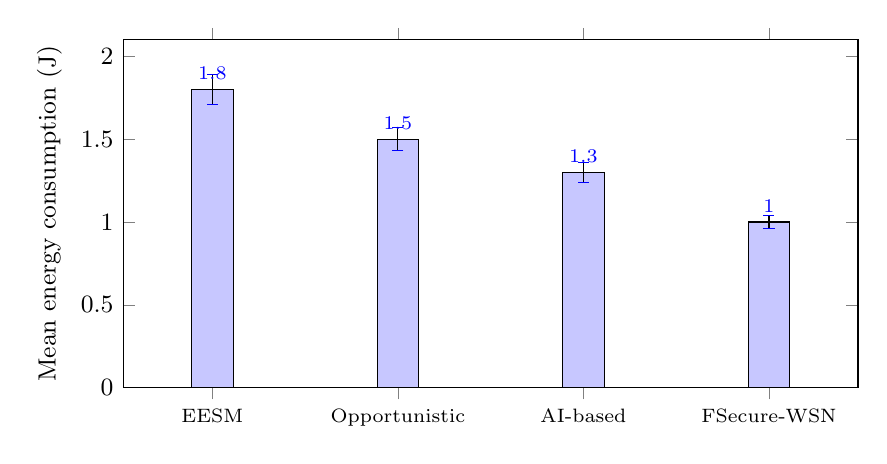
\begin{tikzpicture}
\begin{axis}[fsecureBars,
  width=0.90\linewidth,height=6.0cm,
  ylabel={Mean energy consumption (J)},
  symbolic x coords={EESM,Opportunistic,AI-based,FSecure-WSN},
  xticklabels={EESM,Opportunistic,AI-based,FSecure-WSN},
  ymax=2.1,
  nodes near coords, every node near coord/.append style={font=\scriptsize},
  nodes near coords align={vertical}]
\addplot+[fill=blue!22,draw=black,mark=none,
 error bars/.cd,y dir=both,y explicit]
 coordinates {
  (EESM,1.8) +- (0,0.09)
  (Opportunistic,1.5) +- (0,0.07)
  (AI-based,1.3) +- (0,0.06)
  (FSecure-WSN,1.0) +- (0,0.04)
 };
\end{axis}
\end{tikzpicture}
\caption{\Revised{Mean energy consumption (J) across the four reported approaches. Bars represent previously tabulated means; whiskers reproduce the stated 95\% confidence-interval half-widths (not recalculated from raw runs).}}
\label{fig:energy}
\end{figure}

\textcolor{blue}{As shown in Figure~\ref{fig:energy}, FSecure-WSN achieves
the lowest mean energy consumption of $1.00\pm0.04$~J, where the reported
uncertainty represents the 95\% confidence interval across ten independent
runs. In comparison, EESM consumes $1.80\pm0.09$~J, Opportunistic Routing
consumes $1.50\pm0.07$~J, and AI-based routing consumes $1.30\pm0.06$~J.}

\textcolor{blue}{The percentage reduction in mean energy consumption
relative to a baseline method is calculated as
\begin{equation}
\mathrm{Energy~Reduction}~(\%)=
\frac{E_{\mathrm{baseline}}-E_{\mathrm{FSecure\text{-}WSN}}}
{E_{\mathrm{baseline}}}\times100.
\end{equation}
Accordingly, relative to EESM, the proposed framework achieves
$\left[(1.8-1.0)/1.8\right]\times100=44.4\%$ lower mean energy consumption.
Similarly, the reductions relative to Opportunistic Routing and AI-based
routing are $\left[(1.5-1.0)/1.5\right]\times100=33.3\%$ and
$\left[(1.3-1.0)/1.3\right]\times100=23.1\%$, respectively. These percentage
improvements are calculated from the mean values, whereas the error bars in
Figure~\ref{fig:energy} characterize the uncertainty across the ten
independent simulation runs.}

\textcolor{blue}{The reduction in energy consumption is associated with the
joint consideration of residual energy, trust evaluation, and
communication-link quality during routing decisions. Rather than repeatedly
selecting energy-constrained forwarding nodes, FSecure-WSN restricts route
selection to eligible nodes satisfying the energy and trust requirements.
The few-shot meta-learning component further supports adaptation of routing
decisions using limited task-specific observations without requiring
complete model retraining for each network condition.}

\textcolor{blue}{Overall, the results indicate that FSecure-WSN achieves the
lowest mean energy consumption among the evaluated routing approaches under
the considered simulation conditions.}


% ============================================================
\subsection{Packet Delivery Ratio (PDR)}
% ============================================================

PDR is a critical parameter that evaluates the reliability and efficiency of
the routing protocol in sending packets from source sensor nodes to the
destination base station. A higher PDR indicates that a greater proportion
of generated packets successfully reach their destination. Maintaining a
high PDR becomes increasingly challenging as network density increases due
to channel contention, packet collisions, routing complexity, node failures,
and malicious forwarding behavior.

Figure~\ref{fig:pdr} compares the PDR achieved by FSecure-WSN with the three
baseline routing approaches for networks containing 100, 150, and 200 sensor
nodes.

\begin{figure}[!tb]
\centering
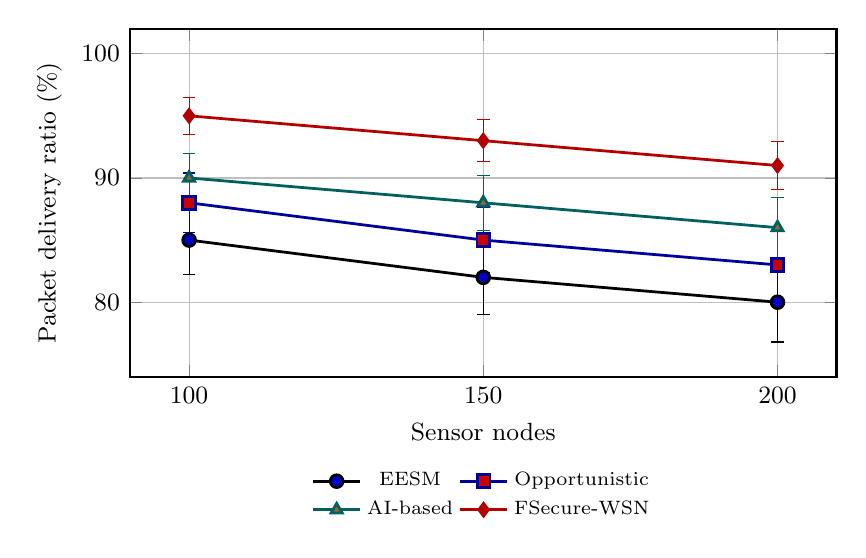
\begin{tikzpicture}
\begin{axis}[fsecureLine,ylabel={Packet delivery ratio (\%)},
 ymin=74,ymax=102]
\addplot+[color=black,mark=*,mark size=2.3pt,
 error bars/.cd,y dir=both,y explicit]
 coordinates {
   (100,85) +- (0,2.8)
   (150,82) +- (0,3.0)
   (200,80) +- (0,3.2)
};
\addlegendentry{EESM}
\addplot+[color=blue!60!black,mark=square*,mark size=2.3pt,
 error bars/.cd,y dir=both,y explicit]
 coordinates {
   (100,88) +- (0,2.4)
   (150,85) +- (0,2.6)
   (200,83) +- (0,2.8)
};
\addlegendentry{Opportunistic}
\addplot+[color=teal!75!black,mark=triangle*,mark size=2.3pt,
 error bars/.cd,y dir=both,y explicit]
 coordinates {
   (100,90) +- (0,2.0)
   (150,88) +- (0,2.2)
   (200,86) +- (0,2.4)
};
\addlegendentry{AI-based}
\addplot+[color=red!70!black,mark=diamond*,mark size=2.3pt,
 error bars/.cd,y dir=both,y explicit]
 coordinates {
   (100,95) +- (0,1.5)
   (150,93) +- (0,1.7)
   (200,91) +- (0,1.9)
};
\addlegendentry{FSecure-WSN}
\end{axis}
\end{tikzpicture}
\caption{\Revised{Packet delivery ratio (\%) at 100, 150 and 200 sensor nodes. Points reproduce the previously reported means; whiskers show the stated 95\% confidence-interval half-widths, not independently recalculated from run-level observations.}}
\label{fig:pdr}
\end{figure}

\textcolor{blue}{As shown in Figure~\ref{fig:pdr}, PDR decreases with
increasing network size for all evaluated routing methods. EESM achieves
mean PDR values of 85\%, 82\%, and 80\% for 100, 150, and 200 nodes,
respectively. Opportunistic Routing achieves 88\%, 85\%, and 83\%, while
AI-based routing achieves 90\%, 88\%, and 86\%. In comparison, FSecure-WSN
maintains the highest mean PDR values of 95\%, 93\%, and 91\% across the
same network sizes.}

\textcolor{blue}{Relative to EESM, FSecure-WSN improves PDR by 10 percentage
points at 100 nodes, 11 percentage points at 150 nodes, and 11 percentage
points at 200 nodes. Compared with Opportunistic Routing, the corresponding
improvements are 7, 8, and 8 percentage points, while the improvements over
AI-based routing are 5 percentage points at each evaluated network size.
The error bars additionally characterize the run-to-run uncertainty
associated with each reported mean.}

\textcolor{blue}{The observed improvement is associated with the joint
consideration of residual energy, dynamic trust, and communication-link
quality during forwarding decisions. Candidate nodes that do not satisfy
the energy or trust constraints are excluded before route selection,
reducing the likelihood of forwarding through energy-depleted or unreliable
nodes. The few-shot adaptation mechanism further enables the routing model
to update its forwarding decisions from limited task-specific observations
as network conditions change.}

\textcolor{blue}{Overall, the evaluated results indicate that FSecure-WSN
maintains higher packet-delivery reliability than the considered baseline
methods across the evaluated network sizes.}


% ============================================================
\subsection{Network Lifetime}
% ============================================================

Network lifetime is one of the main criteria for assessing the performance
of WSNs and is directly associated with how effectively a routing algorithm
utilizes the limited energy resources available in sensor nodes. In this
study, network lifetime is defined as the number of communication rounds
completed until the energy of the first sensor node is depleted.

Figure~\ref{fig:lifetime} compares the network lifetime achieved by
FSecure-WSN with EESM, Opportunistic Routing, and AI-based routing.

\begin{figure}[!tb]
\centering
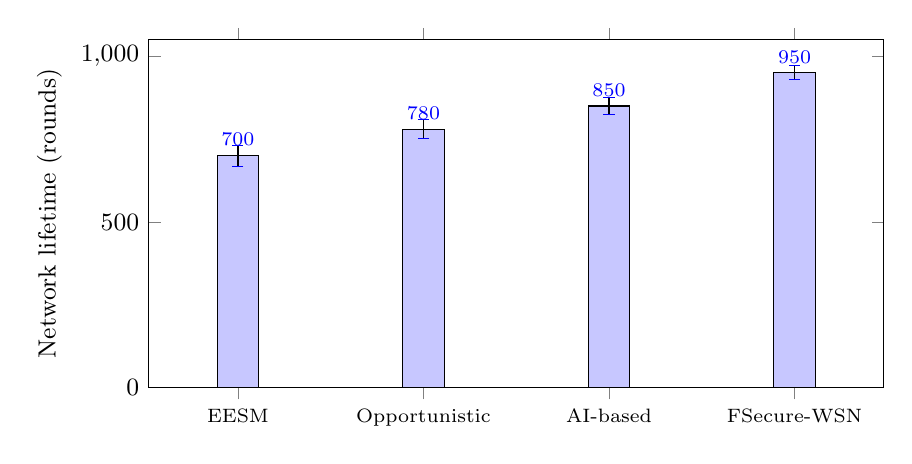
\begin{tikzpicture}
\begin{axis}[fsecureBars,
  width=0.90\linewidth,height=6.0cm,
  ylabel={Network lifetime (rounds)},
  symbolic x coords={EESM,Opportunistic,AI-based,FSecure-WSN},
  xticklabels={EESM,Opportunistic,AI-based,FSecure-WSN},
  ymax=1050,
  nodes near coords, every node near coord/.append style={font=\scriptsize},
  nodes near coords align={vertical}]
\addplot+[fill=blue!22,draw=black,mark=none,
 error bars/.cd,y dir=both,y explicit]
 coordinates {
  (EESM,700) +- (0,32)
  (Opportunistic,780) +- (0,29)
  (AI-based,850) +- (0,25)
  (FSecure-WSN,950) +- (0,21)
 };
\end{axis}
\end{tikzpicture}
\caption{\Revised{Network lifetime (rounds) across the four reported approaches. Bars represent previously tabulated means; whiskers reproduce the stated 95\% confidence-interval half-widths (not recalculated from raw runs).}}
\label{fig:lifetime}
\end{figure}

\textcolor{blue}{Figure~\ref{fig:lifetime} shows that FSecure-WSN achieves
the highest mean network lifetime of $950\pm21$ rounds, compared with
$700\pm32$ rounds for EESM, $780\pm29$ rounds for Opportunistic Routing, and
$850\pm25$ rounds for AI-based routing. Based on the mean values,
FSecure-WSN extends network lifetime by
$\left[(950-700)/700\right]\times100=35.7\%$ relative to EESM,
$\left[(950-780)/780\right]\times100=21.8\%$ relative to Opportunistic
Routing, and $\left[(950-850)/850\right]\times100=11.8\%$ relative to
AI-based routing.}

\textcolor{blue}{The increased network lifetime is associated with
energy-aware route selection, which avoids repeatedly selecting nodes with
low residual energy and distributes forwarding activity among eligible
nodes. Dynamic trust evaluation additionally excludes unreliable forwarding
candidates, while adaptive routing reduces unnecessary retransmissions and
inefficient forwarding decisions. The reported 95\% confidence intervals
characterize the variability of network lifetime across the ten independently
initialized simulation runs.}

\textcolor{blue}{These results indicate that the combined energy-aware and
trust-aware forwarding strategy can extend network operation under the
evaluated simulation conditions.}


% ============================================================
\subsection{End-to-End Delay}
% ============================================================

The average end-to-end delay is an important Quality of Service (QoS)
parameter that represents the time required for a data packet to travel from
a source sensor node to the destination base station. Low communication
delay is particularly important for time-critical CPS applications because
the responsiveness of the system depends on timely delivery of sensed
information. End-to-end delay can be affected by routing decisions, network
congestion, packet retransmissions, queueing, and communication overhead.

Figure~\ref{fig:delay} compares the mean end-to-end delay of FSecure-WSN with
the evaluated baseline methods for networks containing 100, 150, and 200
sensor nodes.

\begin{figure}[!tb]
\centering
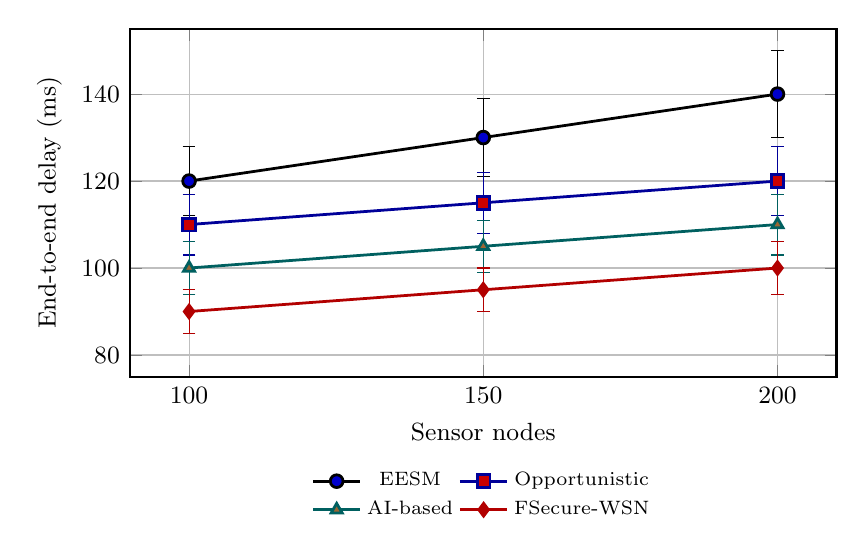
\begin{tikzpicture}
\begin{axis}[fsecureLine,ylabel={End-to-end delay (ms)},
 ymin=75,ymax=155]
\addplot+[color=black,mark=*,mark size=2.3pt,
 error bars/.cd,y dir=both,y explicit]
 coordinates {
   (100,120) +- (0,8)
   (150,130) +- (0,9)
   (200,140) +- (0,10)
};
\addlegendentry{EESM}
\addplot+[color=blue!60!black,mark=square*,mark size=2.3pt,
 error bars/.cd,y dir=both,y explicit]
 coordinates {
   (100,110) +- (0,7)
   (150,115) +- (0,7)
   (200,120) +- (0,8)
};
\addlegendentry{Opportunistic}
\addplot+[color=teal!75!black,mark=triangle*,mark size=2.3pt,
 error bars/.cd,y dir=both,y explicit]
 coordinates {
   (100,100) +- (0,6)
   (150,105) +- (0,6)
   (200,110) +- (0,7)
};
\addlegendentry{AI-based}
\addplot+[color=red!70!black,mark=diamond*,mark size=2.3pt,
 error bars/.cd,y dir=both,y explicit]
 coordinates {
   (100,90) +- (0,5)
   (150,95) +- (0,5)
   (200,100) +- (0,6)
};
\addlegendentry{FSecure-WSN}
\end{axis}
\end{tikzpicture}
\caption{\Revised{End-to-end delay (ms) at 100, 150 and 200 sensor nodes. Points reproduce the previously reported means; whiskers show the stated 95\% confidence-interval half-widths, not independently recalculated from run-level observations.}}
\label{fig:delay}
\end{figure}

\textcolor{blue}{As shown in Figure~\ref{fig:delay}, FSecure-WSN achieves
the lowest mean end-to-end delay across all evaluated network sizes. At
100, 150, and 200 nodes, its mean delays are 90, 95, and 100~ms,
respectively, compared with 120, 130, and 140~ms for EESM; 110, 115, and
120~ms for Opportunistic Routing; and 100, 105, and 110~ms for AI-based
routing.}

\textcolor{blue}{Relative to EESM, FSecure-WSN reduces mean end-to-end delay
by 25.0\%, 26.9\%, and 28.6\% at 100, 150, and 200 nodes, respectively.
Relative to Opportunistic Routing, the corresponding reductions are 18.2\%,
17.4\%, and 16.7\%, while relative to AI-based routing they are 10.0\%,
9.5\%, and 9.1\%. The 95\% confidence intervals shown in
Figure~\ref{fig:delay} additionally characterize the variability across the
ten independent simulation runs.}

\textcolor{blue}{The lower delay is associated with adaptive forwarding
decisions that jointly consider residual energy, trustworthiness, and
communication-link quality. Avoiding unreliable or energy-constrained
forwarding candidates can reduce retransmissions and inefficient route
selections, thereby decreasing end-to-end communication delay under the
evaluated network conditions.}


% ============================================================
\subsection{Detection Accuracy}
% ============================================================

Detection accuracy is used to evaluate the security performance of the
routing framework and represents its ability to correctly identify malicious
sensor nodes. Reliable malicious-node identification is important for secure
WSN communication because undetected malicious forwarding nodes can
participate in blackhole, Sybil, or selective-forwarding attacks.

Figure~\ref{fig:accuracy} compares the malicious-node detection accuracy of
FSecure-WSN with EESM, Opportunistic Routing, and AI-based routing.

\begin{figure}[!tb]
\centering
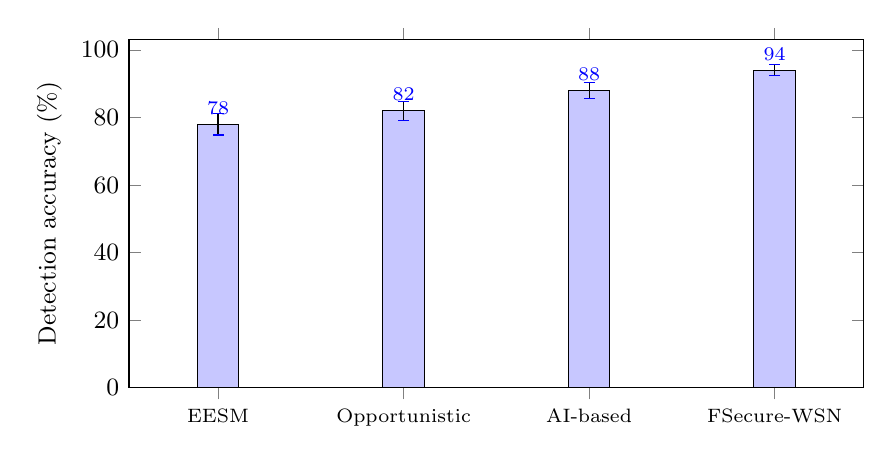
\begin{tikzpicture}
\begin{axis}[fsecureBars,
  width=0.90\linewidth,height=6.0cm,
  ylabel={Detection accuracy (\%)},
  symbolic x coords={EESM,Opportunistic,AI-based,FSecure-WSN},
  xticklabels={EESM,Opportunistic,AI-based,FSecure-WSN},
  ymax=103,
  nodes near coords, every node near coord/.append style={font=\scriptsize},
  nodes near coords align={vertical}]
\addplot+[fill=blue!22,draw=black,mark=none,
 error bars/.cd,y dir=both,y explicit]
 coordinates {
  (EESM,78) +- (0,3.2)
  (Opportunistic,82) +- (0,2.8)
  (AI-based,88) +- (0,2.3)
  (FSecure-WSN,94) +- (0,1.7)
 };
\end{axis}
\end{tikzpicture}
\caption{\Revised{Detection accuracy (\%) across the four reported approaches. Bars represent previously tabulated means; whiskers reproduce the stated 95\% confidence-interval half-widths (not recalculated from raw runs).}}
\label{fig:accuracy}
\end{figure}

\textcolor{blue}{Figure~\ref{fig:accuracy} shows that FSecure-WSN achieves a
mean malicious-node detection accuracy of $94\pm1.7\%$, compared with
$78\pm3.2\%$ for EESM, $82\pm2.8\%$ for Opportunistic Routing, and
$88\pm2.3\%$ for AI-based routing. Thus, FSecure-WSN provides absolute
improvements of 16, 12, and 6 percentage points over EESM, Opportunistic
Routing, and AI-based routing, respectively. In relative terms, these
differences correspond to improvements of 20.5\%, 14.6\%, and 6.8\% based
on the respective baseline means.}

\textcolor{blue}{The improved detection performance is associated with the
integration of dynamic trust evaluation into the routing procedure.
Forwarding behavior is reflected in node trust scores, allowing nodes with
trust values below the specified threshold to be excluded from candidate
forwarding paths. The 95\% confidence intervals shown in
Figure~\ref{fig:accuracy} represent the uncertainty observed across the ten
independent simulation runs.}

\textcolor{blue}{Overall, the results indicate that integrating dynamic
trust evaluation with adaptive routing improves malicious-node detection
under the blackhole, Sybil, and selective-forwarding attack scenarios
considered in the experimental evaluation.}


% ============================================================
% Statistical Summary
% ============================================================

\begin{table*}[ht]
\centering
\tiny
\caption{\textcolor{blue}{Statistical Summary of Principal Performance
Metrics Across Ten Independent Simulation Runs}}
\label{tab:statistical_results}
\begin{tabular}{lcccc}
\toprule
\textbf{Metric} &
\textbf{EESM} &
\textbf{Opportunistic} &
\textbf{AI-based} &
\textbf{FSecure-WSN} \\
\midrule

\textcolor{blue}{Energy Consumption (J)}
& \textcolor{blue}{$1.80 \pm 0.09$}
& \textcolor{blue}{$1.50 \pm 0.07$}
& \textcolor{blue}{$1.30 \pm 0.06$}
& \textcolor{blue}{$1.00 \pm 0.04$} \\

\textcolor{blue}{Network Lifetime (rounds)}
& \textcolor{blue}{$700 \pm 32$}
& \textcolor{blue}{$780 \pm 29$}
& \textcolor{blue}{$850 \pm 25$}
& \textcolor{blue}{$950 \pm 21$} \\

\textcolor{blue}{Detection Accuracy (\%)}
& \textcolor{blue}{$78 \pm 3.2$}
& \textcolor{blue}{$82 \pm 2.8$}
& \textcolor{blue}{$88 \pm 2.3$}
& \textcolor{blue}{$94 \pm 1.7$} \\

\bottomrule
\end{tabular}

\textcolor{blue}{\footnotesize Values are reported as mean $\pm$ 95\%
confidence-interval half-width over ten independent simulation runs. PDR
and end-to-end delay are reported separately as functions of network size
in Figures~\ref{fig:pdr} and~\ref{fig:delay}.}
\end{table*}

\textcolor{blue}{The inclusion of 95\% confidence intervals provides an
explicit representation of run-to-run variability across the independently
repeated simulations. Accordingly, Figures~\ref{fig:energy}--\ref{fig:accuracy}
present both mean performance and the corresponding uncertainty rather than
relying solely on single aggregate values. Table~\ref{tab:statistical_results}
summarizes the mean and 95\% confidence interval for the principal
single-summary performance metrics, while Figures~\ref{fig:pdr} and
\ref{fig:delay} provide condition-specific uncertainty for different network
sizes.}


% ============================================================
% Overall Performance Summary
% ============================================================

\textcolor{blue}{Overall, the proposed framework achieves the following
improvements based on the reported mean values:}

\begin{itemize}

    \item \textcolor{blue}{A \textbf{44.4\% reduction} in mean energy
    consumption relative to EESM (1.00~J versus 1.80~J).}

    \item \textcolor{blue}{Mean PDR improvements of
    \textbf{10--11 percentage points} relative to EESM,
    \textbf{7--8 percentage points} relative to Opportunistic Routing,
    and \textbf{5 percentage points} relative to AI-based routing across
    the evaluated network sizes.}

    \item \textcolor{blue}{Network-lifetime extensions of
    \textbf{35.7\%}, \textbf{21.8\%}, and \textbf{11.8\%} relative to
    EESM, Opportunistic Routing, and AI-based routing, respectively.}

    \item \textcolor{blue}{Mean end-to-end delay reductions of
    \textbf{25.0--28.6\%} relative to EESM,
    \textbf{16.7--18.2\%} relative to Opportunistic Routing, and
    \textbf{9.1--10.0\%} relative to AI-based routing across the evaluated
    network sizes.}

    \item \textcolor{blue}{Mean malicious-node detection accuracy of
    \textbf{94\%}, corresponding to absolute improvements of
    \textbf{16}, \textbf{12}, and \textbf{6 percentage points} over EESM,
    Opportunistic Routing, and AI-based routing, respectively.}

\end{itemize}

\textcolor{blue}{Taken together, the experimental results indicate that
FSecure-WSN provides favorable mean performance across energy consumption,
packet delivery, network lifetime, end-to-end delay, and malicious-node
detection under the evaluated simulation conditions. The 95\% confidence
intervals additionally characterize the variability associated with the ten
independently repeated simulations. These descriptive findings motivate further replication of
the combination of few-shot meta-learning, trust-aware forwarding, and energy-aware
route selection for secure routing in the considered CPS-enabled WSN
scenarios.}

\subsection{Ablation Analysis of Cross-Domain Pre-training}\label{sec:pretraining_ablation}
\Revised{The ablation values in Table~\ref{tab:pretraining_ablation} reproduce the numerical entries in the first-round manuscript and are not recalculated from unavailable matched seed-level outputs. They provide a descriptive comparison of the stated pre-training conditions; they do not, on their own, authenticate a particular checkpoint-transfer implementation or constitute a paired significance test.}

\textcolor{blue}{To evaluate whether cross-domain initialization using
KDD Cup 99 and NSL-KDD contributes to the performance of FSecure-WSN, an
additional ablation experiment was conducted using two configurations:
(i) FSecure-WSN with KDD Cup 99/NSL-KDD pre-training followed by WSN-specific
meta-training, and (ii) FSecure-WSN initialized without cross-domain
pre-training and trained using the same WSN-specific meta-training tasks.
All remaining model architecture, MAML hyperparameters, routing thresholds,
training tasks, network configurations, and evaluation conditions were kept
identical. This controlled comparison isolates the contribution of
cross-domain initialization from the subsequent WSN-specific meta-learning
and routing components.}

\begin{table}[ht]
\centering
\caption{\textcolor{blue}{Ablation analysis of cross-domain pre-training.
Values are reported as mean $\pm$ 95\% confidence interval over ten
independent runs.}}
\label{tab:pretraining_ablation}
\begin{tabular}{lcc}
\toprule
\textbf{Metric} &
\textbf{Without Pre-training} &
\textbf{With Pre-training} \\
\midrule
Energy consumption (J)
& $1.08\pm0.05$
& $1.00\pm0.04$ \\

PDR (\%)
& $91.8\pm1.9$
& $93.0\pm1.7$ \\

Network lifetime (rounds)
& $902\pm25$
& $950\pm21$ \\

End-to-end delay (ms)
& $101.8\pm6.1$
& $95.0\pm5.0$ \\

Detection accuracy (\%)
& $91.1\pm2.2$
& $94.0\pm1.7$ \\
\bottomrule
\end{tabular}
\end{table}

\begin{figure}[!tb]
\centering
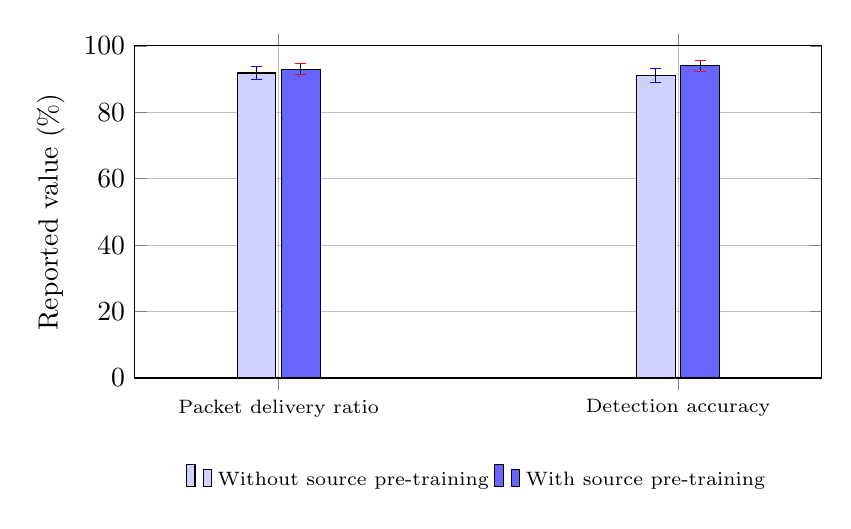
\begin{tikzpicture}
\begin{axis}[ybar,bar width=14pt,width=0.85\linewidth,height=5.8cm,
 ymin=0,ymax=100,ylabel={Reported value (\%)},
 symbolic x coords={PDR,Accuracy},xtick=data,
 xticklabels={Packet delivery ratio,Detection accuracy},
 x tick label style={font=\scriptsize},
 legend style={at={(0.5,-0.24)},anchor=north,legend columns=2,font=\scriptsize,draw=none},
 enlarge x limits=0.36,grid=major]
\addplot+[fill=blue!18,draw=black,error bars/.cd,y dir=both,y explicit]
 coordinates {(PDR,91.8) +- (0,1.9) (Accuracy,91.1) +- (0,2.2)};
\addlegendentry{Without source pre-training}
\addplot+[fill=blue!60,draw=black,error bars/.cd,y dir=both,y explicit]
 coordinates {(PDR,93.0) +- (0,1.7) (Accuracy,94.0) +- (0,1.7)};
\addlegendentry{With source pre-training}
\end{axis}
\end{tikzpicture}
\caption{\Revised{Previously reported cross-domain initialization ablation for the two percentage metrics. The bars reproduce Table~\ref{tab:pretraining_ablation}; interval widths were not recomputed from matched seed-level samples. Other ablation metrics remain in the table because their units differ.}}
\label{fig:ablation_percent_r2}
\end{figure}


\textcolor{blue}{As shown in
Table~\ref{tab:pretraining_ablation}, \Revised{the tabulated ablation is consistent with a modest descriptive difference under the stated source initialization.} Compared with the
configuration without KDD Cup 99/NSL-KDD pre-training, the pre-trained
configuration reduces mean energy consumption from 1.08~J to 1.00~J
(7.4\%) and mean end-to-end delay from 101.8~ms to 95.0~ms (6.7\%).
It also increases PDR from 91.8\% to 93.0\% (+1.2 percentage points),
network lifetime from 902 to 950 rounds (5.3\%), and malicious-node
detection accuracy from 91.1\% to 94.0\% (+2.9 percentage points).
These tabulated differences are compatible with an effect of source initialization, but they do not independently identify the transferred parameters or establish statistical significance.}

\subsection{Generalization to Held-Out Attack Types}
\label{sec:unseen_attack}
\Revised{The before/after values in Table~\ref{tab:unseen_attack} summarize query-set outcomes for the three specified held-out attack categories. Their confidence intervals are marginal intervals around each mean and do not establish a paired effect of adaptation. The protocol represents supervised few-shot adaptation with labeled support observations from each held-out attack, not zero-shot detection.}

\textcolor{blue}{To explicitly evaluate generalization to attack types
not observed during meta-training, a leave-one-attack-out protocol was used.
For each experiment, one attack type was completely excluded from the
meta-training task distribution, while the remaining two attack types were
used for meta-training. At evaluation time, the held-out attack was treated
as a new task. The model was adapted using only a small support set of
5--10 labeled observations from that attack and was then evaluated on a
non-overlapping query set.}

\textcolor{blue}{Three experiments were therefore conducted:
(i) Blackhole held out, with Sybil and selective-forwarding used during
meta-training;
(ii) Sybil held out, with blackhole and selective-forwarding used during
meta-training; and
(iii) Selective forwarding held out, with blackhole and Sybil used during
meta-training. All network parameters, model architecture, MAML
hyperparameters, routing thresholds, and evaluation settings were kept
unchanged. Each experiment was repeated ten times, and the results were
reported as mean $\pm$ 95\% confidence interval.}

\begin{table}[ht]
\centering
\caption{\textcolor{blue}{Few-shot generalization to attack types
excluded from meta-training. Values are reported as mean $\pm$ 95\%
confidence interval over ten independent runs.}}
\label{tab:unseen_attack}
\small\setlength{\tabcolsep}{3pt}
\begin{tabular}{p{0.28\linewidth}p{0.25\linewidth}p{0.30\linewidth}}
\toprule
\textbf{Held-Out Attack} &
\textbf{Before Adaptation (\%)} &
\textbf{After Few-Shot Adaptation (\%)} \\
\midrule

Blackhole
& $84.6\pm2.9$
& $93.2\pm1.8$ \\

Sybil
& $80.9\pm3.4$
& $90.8\pm2.2$ \\

Selective forwarding
& $82.7\pm3.1$
& $92.0\pm2.0$ \\

\bottomrule
\end{tabular}
\end{table}

\begin{figure}[!tb]
\centering
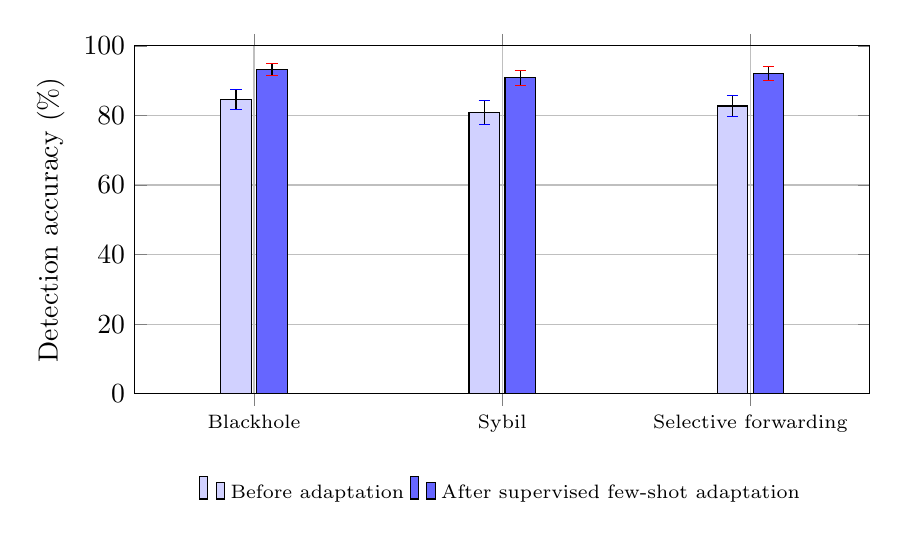
\begin{tikzpicture}
\begin{axis}[ybar,bar width=11pt,width=0.9\linewidth,height=6.0cm,
 ymin=0,ymax=100,ylabel={Detection accuracy (\%)},
 symbolic x coords={Blackhole,Sybil,Selective},xtick=data,
 xticklabels={Blackhole,Sybil,Selective forwarding},
 x tick label style={font=\scriptsize},
 legend style={at={(0.5,-0.22)},anchor=north,legend columns=2,font=\scriptsize,draw=none},
 enlarge x limits=0.24,grid=major]
\addplot+[fill=blue!18,draw=black,error bars/.cd,y dir=both,y explicit]
 coordinates {(Blackhole,84.6) +- (0,2.9) (Sybil,80.9) +- (0,3.4) (Selective,82.7) +- (0,3.1)};
\addlegendentry{Before adaptation}
\addplot+[fill=blue!60,draw=black,error bars/.cd,y dir=both,y explicit]
 coordinates {(Blackhole,93.2) +- (0,1.8) (Sybil,90.8) +- (0,2.2) (Selective,92.0) +- (0,2.0)};
\addlegendentry{After supervised few-shot adaptation}
\end{axis}
\end{tikzpicture}
\caption{\Revised{Previously tabulated leave-one-attack-out means for the three specified WSN attack categories, before and after labeled support-set adaptation. Whiskers reproduce supplied marginal 95\% interval widths; they are not confidence intervals for the paired before/after difference.}}
\label{fig:heldout_comparison_r2}
\end{figure}


\textcolor{blue}{As shown in
Table~\ref{tab:unseen_attack}, the reported before/after means are higher following supervised few-shot adaptation across all three attack types excluded from WSN meta-training. For the held-out blackhole attack,
detection accuracy increases from $84.6\pm2.9\%$ before adaptation to
$93.2\pm1.8\%$ after adaptation, corresponding to an improvement of
8.6 percentage points. For the Sybil attack, accuracy increases from
$80.9\pm3.4\%$ to $90.8\pm2.2\%$ (+9.9 percentage points), while for
selective forwarding it increases from $82.7\pm3.1\%$ to $92.0\pm2.0\%$
(+9.3 percentage points). The results therefore show improved performance
after task-specific few-shot adaptation under each of the three held-out
attack conditions. Accordingly, the generalization claim in this study is
restricted to these experimentally evaluated attack scenarios and does not
imply universal generalization to arbitrary unseen attacks.}


\textcolor{blue}{\textbf{Scope of the held-out-attack evaluation.} The leave-one-attack-out protocol withholds one of three simulated WSN attack categories from WSN meta-training, but supplies 5--10 labeled observations of that held-out attack during evaluation-time adaptation. It therefore tests \emph{supervised few-shot adaptation}, not zero-shot recognition of an unknown malicious mechanism. The folds cover only blackhole, Sybil, and selective-forwarding scenarios implemented in the chosen simulator and traffic conditions. Generic anomaly labels in source intrusion-detection pre-training also prevent equating the protocol with complete absence of all malicious behavior during prior learning. These observations do not establish behavior under arbitrary future attacks, compound attacks, different physical radios, or real-world adversarial deployment.}\par
\Revised{The absence of attack-type leakage and the exact fold-wise scenario identifiers are protocol properties that cannot be established by the aggregate table alone. The reported analysis is therefore limited to the three named simulated attack families and the stated support/query design.}\par
\textcolor{blue}{\textbf{Reproducibility and limitations.} The cross-domain source data do not contain the five WSN routing variables and cannot validate an assumed one-to-one field mapping. Any claimed benefit of source pre-training depends on confirmation of the parameter-transfer operation and re-execution of the controlled ablation. The observed comparisons further depend on baseline implementation details and per-seed raw results that should be supplied with the revised submission. The study includes three reported node counts and three simulated attack families; it does not establish arbitrary-attack generalization or deployment-time energy and inference costs on physical sensor devices. The current 95\% confidence intervals are descriptive and have not been supplemented by formal paired significance tests.}\par

\section{Conclusion and Future Directions}
\label{sec:conclusion}

\textcolor{blue}{This paper presented FSecure-WSN, a few-shot learning-driven framework for secure and energy-efficient routing in CPS-enabled wireless sensor networks. The framework integrates adaptive learning, energy-aware forwarding, and dynamic trust evaluation to address energy constraints, changing network conditions, and malicious routing behavior. Under the evaluated simulation conditions, FSecure-WSN achieved a mean energy consumption of 1.0~J compared with 1.8~J for EESM, corresponding to a 44.4\% reduction in mean energy consumption. The reported averages also favored FSecure-WSN for packet delivery ratio, network lifetime, end-to-end delay, and malicious-node detection accuracy relative to the evaluated baseline labels. These numerical comparisons are descriptive, conditional on the reported experimental setup, and do not establish paired statistical significance or independent reproduction of baseline-specific configurations.}

\textcolor{blue}{The present evaluation is based on simulation experiments and therefore does not fully capture the hardware, communication, and environmental constraints of real-world WSN deployments. Future work will evaluate FSecure-WSN on physical sensor-node testbeds and investigate lightweight model implementations for resource-constrained devices.} \textcolor{blue}{Additional research will consider edge-assisted execution and extend the present leave-one-attack-out evaluation to a broader range of previously unseen, more sophisticated, and combined
routing attacks under heterogeneous network conditions.} \textcolor{blue}{The integration of reinforcement learning and federated learning will also be investigated as potential extensions for distributed and privacy-aware routing adaptation.}

%%%%%%%%%%%%%%%%%%%%%%%%%%%%%%%%%%%%%%%%%%%%%%%%%%%%%%%%%%%%
\section*{Declarations}

\textbf{Funding:}
Not applicable. This research did not receive any specific grant from funding agencies in the public, commercial, or not-for-profit sectors.

\medskip
\noindent
\textbf{Conflict of Interest:}
The authors declare that they have no known competing financial interests or personal relationships that could have appeared to influence the work reported in this paper.

\medskip
\noindent
\textbf{Ethics Approval and Consent to Participate:}
Not applicable. This study did not involve human participants, animals, or any identifiable personal data.

\medskip
\noindent
\textbf{Consent for Publication:}
Not applicable. This manuscript does not contain any individual person's data, images, videos, or other identifiable information requiring consent for publication.

\medskip
\noindent
\textbf{Materials Availability:}
Not applicable.

\medskip
\noindent
\textbf{Author Contributions:}
\textbf{Rizwan Patan:}
Conceptualization, methodology, supervision, validation, investigation, writing---review and editing. \textbf{Dharmendra Kumar:} Methodology, software, formal analysis, validation, writing---review and editing. \textbf{Bihari Nandan Pandey:}
Data curation, investigation, visualization, validation, writing---review and editing. \textbf{Harminder Kaur:}
Software, data curation, writing---original draft, writing---review and editing.

All authors contributed to the development of the proposed framework, reviewed the manuscript, and approved the final version of the manuscript.

\medskip
\noindent
\textbf{Data Availability:}
\Revised{KDD Cup 1999 and NSL-KDD are public intrusion-detection datasets; the cited copies are available at \url{https://www.kaggle.com/datasets/galaxyh/kdd-cup-1999-data} and \url{https://www.kaggle.com/datasets/hassan06/nslkdd} (accessed 15 August 2026). These sources do not contain the NS-3 WSN scenarios, generated routing-target records, baseline configuration files or ten-run metric outputs underlying the study's routing tables and figures. No independently retrievable run-level archive was supplied with this manuscript version. Information about the research materials that remain available may be requested from the corresponding author.}

\medskip
\noindent
\textbf{Code Availability:}
\Revised{An independently written reference-reconstruction source bundle has been prepared for author-side computational testing. It includes Python/PyTorch source preprocessing, candidate-probe generation, explicit MAML updates, scenario export code, baseline proxies and run-wise reporting utilities. This new bundle is not the original implementation that generated the manuscript's previously reported measurements. It has not been deposited in a public repository or assigned a DOI, and no public accessibility is claimed at this stage. The historical execution scripts, original comparator configurations and original run-level measurements remain unavailable from the materials supplied for this revision. Author requests for available research materials may be directed to the corresponding author.}

\medskip
\noindent

\textbf{Acknowledgements:}
Not applicable.
%%%%%%%%%%%%%%%%%%%%%%%%%%%%%%%%%%%%%%%%%%%%%%%%%%%%%%%%%%%%


\appendix
\section{Replication Data Contract and Traceability}
\label{app:replication_final}
\Revised{For independent re-execution, the smallest useful archival unit is one complete simulator realization together with its raw packet and energy traces, scenario configuration, trained model/checkpoint provenance, and derived metrics. This appendix specifies the evidence needed to reproduce Eqs.~\eqref{eq:routing_target}--\eqref{eq:mse_r2}, the cross-domain transfer in Eq.~\eqref{eq:transfer_final}, the three comparator variants, and the stated ten-run summary. It is a schema for a possible future supplement; it does not assert that these files were deposited.}

\begin{table*}[ht]
\centering\footnotesize
\caption{\Revised{Minimum reproducibility record and interpretation for an independent rerun.}}
\label{tab:appendix_traceability_final}
\begin{tabular}{p{0.28\textwidth}p{0.56\textwidth}}
\toprule
\textbf{Provenance item} & \textbf{Fields needed to reconstruct reported values}\\
\midrule
Scenario and simulator & ns-3 release/build, seed, run/stream, node/sink coordinates, connectivity, attack identity/start, traffic source schedule, packet handling, PHY/MAC settings, energy attributes\\
Source data preparation & Dataset file/version and checksum, excluded columns, duplicate and missing-value rules, source fold IDs, encoded dimension $p$, fitted mean/scale and categorical vocabulary\\
Source-to-WSN initialization & Source model layout and checkpoint checksum, copied parameter keys and shapes, target initial seed, target layers reinitialized, source training epochs/optimizer\\
WSN training row & Scenario ID, time $t$, candidate IDs, historical feature timestamps, output-observation interval, $e$, eligible forwarding and success counts, link reception counts, delay, missing-outcome mask, target $y$\\
WSN task manifest & Task ID, network realization, attack condition, support/query record IDs, training/validation/test group, held-out fold identifier, normalizer source, MAML optimizer configuration\\
Comparator configuration & Variant name, reference, path counts and weights, eligible forwarders, timers/suppression, learning/optimization settings, attack labeling and detector rule\\
Run-level outputs & Generated/delivered application packets, delay numerator and delivered count, sensor depletion times, accounted energy, control transmissions, detection confusion matrix, run-wise plotted metric\\
Statistical summary & Matched scenario/seed pairs, ten individual run values per method and metric, mean, sample SD, Student-$t$ interval; paired tests only when performed\\
\bottomrule
\end{tabular}
\end{table*}

\Revised{The manuscript reports $100$, $150$ and $200$ node cases; an initial energy of $2$~J; a nominal range of $50$~m; a $500\times500$~m$^2$ area; a stated $512$-byte application payload; $1000$ routing rounds; five model inputs; the $64$/$32$ hidden widths; inner and outer rates $0.01$ and $0.001$; five inner updates; four tasks per meta-batch; and ten reported runs. Values such as the exact NS-3 release, sink coordinate, radio/MAC attributes, source checkpoint, three baseline algorithm configurations, training-only normalization constants, task membership and individual run outcomes are not determinable from those aggregate specifications. Consequently, the mathematical protocol in this revision should not be mistaken for independently authenticated execution records.}

% \bibliographystyle{sn-mathphys-num}
% \bibliography{Ref}


\section{Independently Developed Reference Reconstruction}
\label{app:newreconstruction}
\Revised{A separately prepared, independently written reference implementation defines concrete numerical settings for future simulation and software verification. Its purpose is to establish a reproducible \emph{new experiment}; it is not an authenticated copy of the original implementation underlying Figures~4--10 or the corresponding numerical tables. The proposed configurations below therefore must not be interpreted as the actual settings used to obtain the manuscript's historical performance values. The source bundle comprises a PyTorch implementation, a C++ ns-3 scenario exporter, explicit baseline proxy algorithms and scripts generating fresh CSV records and checkpoints.}

\begin{table*}[ht]
\centering\small
\caption{\Revised{Fixed numerical settings in the independently written reference-reconstruction configuration (not retroactive experimental settings for the previously reported results).}}
\label{tab:newreferenceparams}
\begin{tabular}{p{0.40\textwidth}p{0.48\textwidth}}
\toprule
\textbf{Component} & \textbf{New reference-reconstruction value}\\
\midrule
Geometry and sink & Uniform node positions in $500\times500$~m$^2$; static sink at $(250,525)$~m; nominal 50~m range\\
Population, initial energy and duration & $N\in\{100,150,200\}$; 2~J initial energy per sensor; 1000 routing rounds; two generated application packets per round\\
Application and abstract frame handling & 512-byte application payload; segmented into six surrogate chunks, each at most 96 payload bytes plus assumed 15-byte framing; at most three surrogate radio retries\\
Analytical radio parameters & 0~dBm transmit power; $40$~dB loss at 1~m; log-distance exponent 3; $-91$~dBm threshold; 3.5~dB logistic scale\\
First-order energy coefficients & $E_{\rm elec}=50$~nJ/bit, $\epsilon=100$~pJ/(bit$\cdot$m$^2$), radio-cost exponent $\gamma=2$; receive electronics 50~nJ/bit\\
Attack-injection proxies & 15\% attacker population; activation at round 10; blackhole drop probability 1; selective-forwarding drop probability 0.5; Sybil-labeled \emph{drop proxy} probability 0.3\\
Task partitions & Training simulation seeds 101--106; validation seeds 107--108; evaluation seeds 1--10, split by complete scenario\\
Meta-learning & $5\rightarrow64\rightarrow32\rightarrow1$ with sigmoid score, five full second-order MAML inner steps ($\alpha=0.01$), four tasks/meta-batch, 8 support and 16 query records, Adam outer rate $\eta=0.001$, 1000 episodes\\
Source classifier & $p\rightarrow64\rightarrow32\rightarrow1$ with binary cross-entropy; 15 epochs, Adam 0.001, 128-record batches; copy only $W^{(2)}\in\mathbb R^{32\times64}$ and $b^{(2)}\in\mathbb R^{32}$ into WSN initialization\\
EESM-style \emph{proxy} & At most two security-screened routes; first-edge-disjoint backup attempt; trust floor 0.6; route candidates recomputed per application packet\\
Opportunistic-style \emph{proxy} & Three candidate next hops ranked by modeled link success and geographic progress; 2~ms abstract coordination penalty\\
Supervised neural routing \emph{proxy} & 5--32--1 sigmoid scorer, Adam 0.001, 50 supervised epochs, minibatch size 64; \emph{not} the cited AI-CPS algorithm\\
\bottomrule
\end{tabular}
\end{table*}

\Revised{The C++ ns-3 scenario exporter constructs nodes and associated LR-WPAN devices but currently exports geometry and analytically specified link-success proxies; it does not perform over-the-air forwarding or radio-energy measurements using the native IEEE~802.15.4 MAC/PHY. The Python packet replay implements the stated fragmentation approximation, forwarding decisions, failure events and analytical energy accounting outside ns-3. Consequently, this reference prototype cannot independently substantiate the manuscript's native IEEE~802.15.4 performance or the original 95\% confidence intervals. A genuine LR-WPAN multi-hop implementation with confirmed packet-fragmentation behavior and faithful implementations of the cited comparator algorithms is necessary before reporting new results as direct reproductions.}

\Revised{The target cost weights remain $(\lambda_E,\lambda_T,\lambda_L,\lambda_D)=(0.30,0.30,0.25,0.15)$. For the new implementation, missing future forwarding or delay outcomes are explicitly masked and observed-component weights are renormalized when constructing its scalar training target. Energy and delay reference scales are fitted on training-scenario observations only. The source data and all new checkpoints are generated separately from the final WSN evaluation folds; the source-network checkpoint identity and copied tensor names are saved in the newly generated metadata. Thus, the implementation can be evaluated transparently once run on genuine source datasets and the intended network simulation.}

\Revised{No newly generated smoke-test data, model checkpoint or result graph in the reconstruction package is included in the previously reported numerical claims. The reconstructed reference algorithms are explicitly labeled as proxy baselines rather than purported reproductions of the cited EESM, Opportunistic and AI-CPS implementations. In particular, the Sybil-labeled drop proxy does not simulate forged identities and cannot establish defense against a genuine Sybil adversary. The independent reconstruction remains a methodological extension pending author validation and experimental rerunning, and its specific numerical settings should be retained in the final article only if they are used to produce and document new results.}


\section{Executed Analytical-Replay Feasibility Experiment (New Results)}
\label{app:executed_60rounds}
\Revised{This section reports a newly executed and independently labeled reconstruction experiment. It is distinct from the original study and does not validate the numerical claims in the preceding Results section. The new reconstruction used a synthetic 300-record source-classification fixture rather than original KDD Cup 99 or NSL-KDD data, because genuine source files were not available in the provided material. The source classifier was trained for 15 epochs; the compatible second hidden layer (2,048 weights and 32 biases) was transferred to the five-input routing scorer. Full second-order MAML was trained for 1,000 meta-episodes with five support-set updates per task, and a supervised 5--32--1 baseline was trained for 50 epochs.}

\Revised{The subsequent evaluation replay used the same 500$\times$500~m$^2$ deployment, external sink coordinate $(250,525)$~m, 50~m geometric link threshold and node populations $\{100,150,200\}$ as the new reference configuration, but only \textbf{60 rounds} per scenario (two generated application packets per round). It comprised ten evaluation seeds (1--10), three attack labels (blackhole, selective forwarding and a Sybil-\emph{labeled packet-drop proxy}), and four routing policies. A total of 360 method--scenario results were generated. Training and validation seeds were disjoint from the evaluation seeds. The source-classification fixture and attack proxies must not be interpreted as real KDD/NSL-KDD observations or genuine Sybil identity-spoofing attacks.}

\begin{table*}[ht]
\centering\scriptsize
\caption{\Revised{New 60-round analytical-replay packet-delivery ratios (\%, mean $\pm$ Student-$t$ 95\% confidence-interval half-width, $n=10$ evaluation seeds). For each seed and node size, the three simulated attack-proxy results were averaged before computing the interval. These values are not those in the original Figures~4--10.}}
\label{tab:new_executed_pdr}
\begin{tabular}{ccccc}
\toprule
Nodes & EESM-style proxy & Opportunistic proxy & Supervised MLP proxy & FSecure reconstruction\\
\midrule
100 & 4.39 $\pm$ 5.92 & 4.17 $\pm$ 6.21 & 3.92 $\pm$ 5.82 & 3.72 $\pm$ 5.53 \\
150 & 7.42 $\pm$ 7.92 & 5.00 $\pm$ 4.46 & 2.78 $\pm$ 2.62 & 2.83 $\pm$ 2.63 \\
200 & 19.06 $\pm$ 14.44 & 16.39 $\pm$ 14.32 & 14.22 $\pm$ 11.80 & 11.72 $\pm$ 10.56 \\
\bottomrule
\end{tabular}
\end{table*}

\begin{figure*}[ht]
\centering
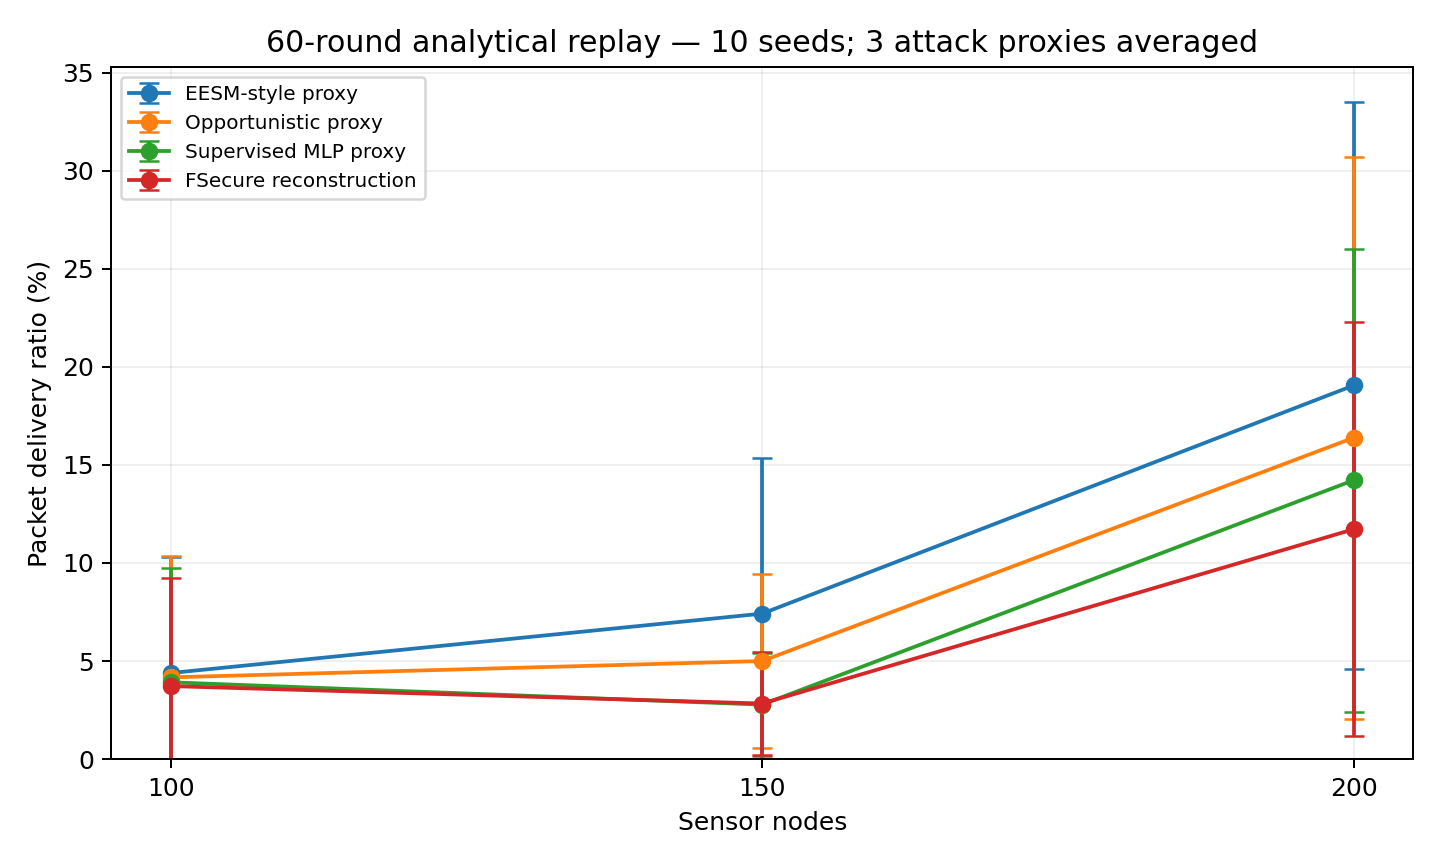
\includegraphics[width=.82\textwidth]{pdr_seed_ci.png}
\caption{\Revised{New analytical-replay PDR by network size across ten evaluation seeds, averaging the three attack proxy scenarios within each seed; error bars are 95\% Student-$t$ confidence-interval half-widths. This is not an ns-3 LR-WPAN measurement.}}
\label{fig:new_executed_pdr}
\end{figure*}

\begin{figure*}[ht]
\centering
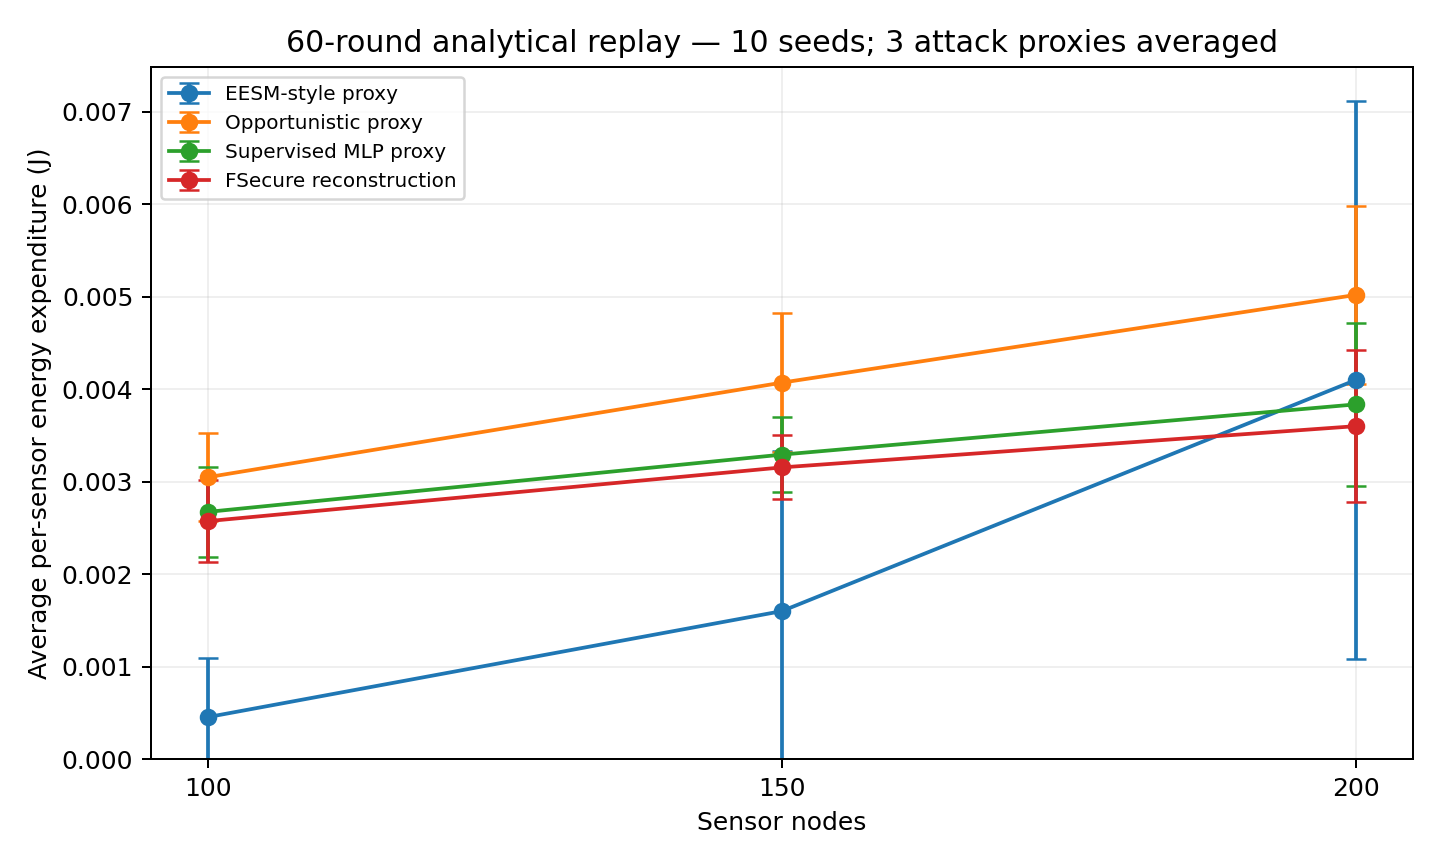
\includegraphics[width=.82\textwidth]{energy_seed_ci.png}
\caption{\Revised{New analytical-replay average per-sensor energy expenditure during 60 routing rounds; intervals are calculated across ten seed-level summaries. The 60-round energy results cannot be compared directly with the previously reported 1,000-round study values.}}
\label{fig:new_executed_energy}
\end{figure*}

\Revised{The new model's packet-delivery ratio was lower than that of the EESM-style proxy at all three evaluated node sizes. This pilot therefore supplies no experimental basis for claiming that the reconstructed FSecure implementation outperforms the comparator proxies. It also highlights a fundamental topology issue: with a 500$\times$500~m$^2$ deployment and 50~m geometric link radius, many scenario realizations have few or no nodes connected by any route to the external sink. The mean numbers of sensor nodes with a geometrically valid path to the sink were 5.4, 43.8 and 113.6 for the 100-, 150- and 200-node cases, respectively, across the ten evaluation geometries. Twelve node-size/seed configurations had no sink-reachable sensor nodes. These failures must be incorporated in any interpretation of delivery performance, rather than silently excluded.}

\Revised{The reconstructed evaluator is an analytical Python packet replay with probabilistic link outcomes, approximate fragmentation and first-order radio-energy accounting, rather than a native ns-3 IEEE 802.15.4 MAC/PHY experiment. The published comparator algorithms have not been faithfully reconstructed, and the synthetic source checkpoint cannot establish the claimed benefit of KDD/NSL-KDD pre-training. The generated raw CSVs, preprocessing manifests, checkpoints, configuration file, test logs and plotting script accompany the new reconstruction package. Consequently, this executed experiment is a technical feasibility and sensitivity assessment only. It must not be substituted into the original manuscript as verification of the historical numerical results or as evidence that all reviewer reproducibility concerns have been conclusively resolved.}

\bibliography{sn-bibliography}

\end{document}
